\documentclass[a4paper, oneside]{discothesis}

\usepackage[utf8]{inputenc}
\usepackage[T1]{fontenc}
\usepackage{graphicx}
\usepackage{float}
\usepackage{cprotect}
\usepackage{listings}
\usepackage{xcolor}
\usepackage{dirtree}
\usepackage[labelfont=bf,font=small,skip=5pt]{caption}

\definecolor{codegreen}{rgb}{0,0.6,0}
\definecolor{codegray}{rgb}{0.5,0.5,0.5}
\definecolor{codepurple}{rgb}{0.58,0,0.82}
\definecolor{backcolour}{rgb}{0.95,0.95,0.92}


\lstdefinestyle{mystyle}{
	backgroundcolor=\color{backcolour},   
	commentstyle=\color{codegreen},
	keywordstyle=\color{magenta},
	numberstyle=\tiny\color{codegray},
	stringstyle=\color{codepurple},
	basicstyle=\ttfamily\footnotesize,
	breakatwhitespace=false,         
	breaklines=true,                 
	captionpos=b,                    
	keepspaces=true,                 
	numbers=left,                    
	numbersep=5pt,                  
	showspaces=false,                
	showstringspaces=false,
	showtabs=false,                  
	tabsize=2
}
\lstset{style=mystyle}


%%%%%%%%%%%%%%%%%%%%%%%%%%%%%%%%%%%%%%%%%%%%%%%%%%%%%%%%%%%%%%%%%%%%%%%%%%%%%%%%%%%%%%%%%%%%%%%%%
% DOCUMENT METADATA

\thesistype{Master's thesis} % Master's thesis, Bachelor's thesis, Semester thesis, Group Project
\title{Near Resonances for Scattering Transmission Problems}

\author{Diego Renner}
\email{drenner@student.ethz.ch}

\institute{Seminar for Applied Mathematics \\[2pt]
	Computational Science and Engineering \\[2pt]
ETH Zürich}

% Optionally, you can put in your own logo here

\supervisors{Prof.\ Dr.\ Ralf Hiptmair}

% Optionally, keywords and categories of the work can be shown (on the Abstract page)
%\keywords{Keywords go here.}
%\categories{ACM categories go here.}

\date{\today}

%%%%%%%%%%%%%%%%%%%%%%%%%%%%%%%%%%%%%%%%%%%%%%%%%%%%%%%%%%%%%%%%%%%%%%%%%%%%%%%%%%%%%%%%%%%%%%%%%

\begin{document}

\frontmatter % do not remove this line
\maketitle
\cleardoublepage

\begin{acknowledgements}
	I would first like to thank my thesis advisor Prof. Dr. Ralf Hiptmair from the Seminar for Applied Mathematics at the ETH Zürich.
	Throughout the thesis Prof. Hiptmair was always available to offer advice when it came to tricky problems while debugging or when I had questions about the underlying theory.
	When problems arose I could count on his understanding, and when milestones were reached there was excitement to be shared.

	I would also like to thank my girlfriend who offered me strong support during all of my studies and especially during the writing of this thesis.
	Her support made the difficult parts more bearable and the good parts even more enjoyable.

	Finally I would like to thank my parents for allowing me to pursue these studies.
	Without them I could not have invested the time and energy that I did, and I wouldn't be where I am at now.
\end{acknowledgements}


\begin{abstract}
	Near resonances that can be observed in transmission problems for the Helmholtz equation are represented by local minima in the singular values of the operators that are used to describe the problems' Boundary Integral Equation (BIE) formulation.
	The goal of this thesis was to use Boundary Element Methods (BEM) to track these singular values and their derivatives in order to find the minima.
	The BEM operators were validated using known solutions to the Helmholtz transmission problem on a sphere.
	For the derivatives of the singular values the extrapolation method was applied for validation.
	Using the Van Wijngaarden-Dekker-Brent method and the first derivative or the Newton-Raphson method and up to the second derivative, the local minima in the singular values could accurately be determined.
\end{abstract}

\tableofcontents

\mainmatter % do not remove this line

% Start writing here
\chapter{Introduction}
In fields such as acoustics, electromagnetism, and fluid dynamics the wave equation commonly arises. 
It's frequency-domain form, the Helmholtz equation, can be stated as $ \Delta u = k^2 n u $. 
Here, and for the continuation of this thesis, $n$ refers to the refraction index, and the wavenumber $k=\omega/c$ is the ratio of the angular frequency and the wave propagation speed in the medium of interest.
We consider an incoming wave $u_i$ and a bounded open Lipschitz domain $\Omega_i \subset \mathbb{R}^d$, with a refraction index $n_i$ differing from the refraction index $n_o=1$ in $\mathbb{R}^d\setminus\Omega_i$, and we want to know the resulting wave in all of $\mathbb{R}^d$. 
This is called the Helmholtz transmission problem.
The behaviour of the resulting wave for different scatterers $\Omega_i$, and especially the occurring resonances, are of interest in material science and engineering as well as mathematics and physics \cite{PhysRevLett.97.206806} \cite{matscat} \cite{emscat}.

In order to solve the Helmholtz transmission problem the Helmholtz equation has to be solved in $\Omega_i$ and in $\mathbb{R}^d\setminus\Omega_i$ separately under consideration of the appropriate boundary and decay conditions.
This can be done analytically only in rare cases such as $\Omega_i$ being a sphere $B_{a}(0)$ of arbitrary radius $a$. 
For more general cases integral equation methods can be applied \cite{doi:10.1137/1.9781611973167}. 
These have the numerical advantage of transforming a n-dimensional problem on an unbounded domain to a (n-1)-dimensional problem on a bounded domain. 
The occurring resonances are represented by local minima in the singular values of the Boundary Integral Operators (BIO) arising from the integral equation methods.

In this thesis the numerical methods of choice for discretizing the integral equations, or more specifically the boundary integral equations, were Boundary Element Methods (BEM).
In these methods the BIOs are discretized using finite dimensional approximations of the actual Hilbert spaces on the boundary of the domain $\Omega_i$.
As can be shown the singular values of these discretized operators converge towards those of the actual operators as the mesh used for discretization becomes finer \cite{svdap}.
This behaviour was used to compute the singular values and later on to find local minima of the singular values with respect to frequency.

The thesis is structured as follows: in chapter two we will first give a brief overview of the theoretical background surrounding the Helmholtz transmission problem and the methods applied in this thesis to solve it.
Then in chapter three we will describe the different algorithms used to solve the Helmholtz transmission problem numerically as well as the methods for finding the singular values of the involved operators, the singular values' derivatives and the zeros of the first derivatives.
In chapter four we will present the validation of the applied numerical methods and then run some computations with the validated algorithms. 
Finally in chapter five we will give a conclusion to the results from chapter four as well as an outlook upon future work.


\chapter{Theoretical Background}
The theoretical part of this thesis is mainly concerned with the Helmholtz equation and it's more specific application the Helmholtz transmission problem.
Since the goal of this thesis was to develop a numerical tool to help analyse the near resonances occurring in the Helmholtz transmission problem these will be described here briefly as well.
First we will give an overview of the Helmholtz equation itself.

\section{The Helmholtz Equation}
As mentioned in the introduction the Helmholtz equation is the time independent form of the wave equation. 
The wave equation can be derived by considering the pressure $P(x,t)$ and the density $\rho(x,t)$ of a vibrating fluid.
Throughout this thesis we will be considering $x \in \mathbb{R}^2$ and $t \in \mathbb{R}$.
Using the following relationships
\begin{align}
	P &= c^2 \rho \\
	\partial_t \rho + \nabla \cdot (\rho P) &= 0 \\
	\rho \partial_t v &= -\nabla P \\
\end{align}
where $c$ is the speed of sound and $v$ the particle velocity in the vibrating fluid,
we can retrieve the wave equation:
\begin{equation}
	\Delta P - \frac{1}{c^2} \frac{\partial^2 P}{\partial t^2} = 0 .
\end{equation}
To transform this into the Helmholtz equation we choose the time-harmonic dependence of the pressure to be of the form $P(x,t) = u(x)e^{-i\omega \sqrt{n} t}$. 
Here $\omega$ is the angular frequency and $n$ is the refraction index of the fluid.
Entering this assumption into (2.5) we get the Helmholtz equation 
\begin{equation}
	\Delta u + k^2nu = 0
\end{equation}
with the wavenumber $k^2=\frac{w^2}{c^2}$. 
We choose the sign of $k$ to be positive since physically speaking the wavenumber measures the number of waves in an interval of length $2\pi$.
When considering different regions with different refraction indices this becomes the Helmholtz transmission problem which we will discuss in the next section.

\section{The Helmholtz Transmission Problem}
The Helmholtz equation models the time independent propagation of a wave inside one medium.
When going from one medium to another one has to solve the Helmholtz transmission problem.
In order to state this problem we first introduce some notation.
We will denote from here on by $\Omega_i$ a bounded open Lipschitz domain with it's refraction index $n_i$.
The exterior region defined as $\mathbb{R} \setminus \overline{\Omega}_i$ will be referred to as $\Omega_o$ and it has the refraction index $n_o$.
For the boundary between the two domains $\Gamma := \partial\Omega_i = \partial\Omega_o$ we define the following trace operators
\begin{align}
	\begin{split}
		\gamma_D^*: H(\Omega_*) &\longrightarrow H^{1/2}(\Gamma) \\
		u &\longrightarrow \gamma_D^*u := u_{|\Gamma} 
	\end{split}
	\\
	\begin{split}
		\gamma_N^*: H(\Delta,\Omega_*) &\longrightarrow H^{-1/2}(\Gamma) \\
		u &\longrightarrow \gamma_N^*u := \nabla u \cdot \mathbf{n}
	\end{split}
\end{align}
The $*$ symbol can be replaced by either $i$ or $o$ when taking the trace from $\Omega_i$ or $\Omega_o$ as the limit must not necessarily be the same. The vector $\mathbf{n}$ denotes the normal unit vector from $\Omega_i$ to $\Omega_o$. 
Throughout the thesis we will be using the definition for the Hilbert and the boundary spaces that are used in \cite{anmcse}.
These two trace operators are commonly referred to as the Dirichlet and the Neumann Trace respectively.
As a shorthand we will be using the Cauchy trace operator $\gamma^* := (\gamma_D^*, \gamma_N^*)^T$.
Using this notation we can now state the Helmholtz transmission problem as follows
\begin{align}
	\Delta u + k^2n_iu &= 0 & \text{ in }& \Omega_i \\
	\Delta u + k^2n_ou &= 0 & \text{ in }& \Omega_o \\
	\gamma^iu &= \gamma^ou & \text{ on }& \Gamma \\
	iku - \frac{du}{dR} &= o(R^{-1/2}) & \text{ as }& R \rightarrow \infty \label{sfrc}.
\end{align}
Here and for the rest of the thesis we define $R := ||x||$.
The equation \ref{sfrc} is called the Sommerfeld radiation condition and it is needed to discard non-physical solutions that include reflection at infinity. 
It is derived using integral equation methods which will be discussed more closely in section \ref{sec:BIEs}.
For solving the equation has to be brought into a more tangible form.
For this we will split $u$ into an incoming and a scattered wave $u = u_{s} + u_{inc}$ in $\Omega_o$ where $u_{inc}$ solves the Helmholtz equation in $\mathbb{R}^2$:
\begin{equation}
	\Delta u_{inc} + k^2n_ou_{inc} = 0 \qquad \text{ in } \mathbb{R}^2. \label{hme1}
\end{equation}
We also define the resulting wave due to the incoming wave as:
\begin{equation}
	u_{res} := 
	\begin{cases}
		u &\text{ in } \Omega_i \\
		u_s &\text{ in } \Omega_o
	\end{cases}
	.
\end{equation}
Using this definition we can now restate the Helmholtz transmission problem as follows:
\begin{align}
	\Delta u_{res} + k^2n_iu_{res} &= 0 & \text{ in }& \Omega_i \label{hme2}\\
	\Delta u_{res} + k^2n_ou_{res} &= 0 & \text{ in }& \Omega_o \label{hme3}\\
	\gamma^iu - \gamma^ou&= \gamma^iu_{inc} = \gamma^ou_{inc} & \text{ on }& \Gamma \label{bc}\\
	iku_{res} - \frac{du_{res}}{dR} &= o(R^{-1/2}) & \text{ as }& R \rightarrow \infty.
\end{align}
In the next section we will show show an example of a case in which these equations can be solved analytically.

\section{Example of an Analytically Solvable Case} \label{sec:asc}
When $\Omega_i$ is a ball $B_a(0)$ of radius $a$ centred around $0$ there exist analytical solutions to the Helmholtz transmission problem. 
To solve the Helmholtz transmission problem we have to solve the Helmholtz equation in three settings. 
These are the ones stated in the equations \ref{hme1}, \ref{hme2}, and \ref{hme3}. 
To do this we will first find a general solution to the Helmholtz equation by separation of variables. 
This means choosing an Ansatz of the form $u(r,\phi)=R(r)\Phi(\phi)$.
Once we found a general solution using separation of variables we will then go on to fitting it to the appropriate conditions for the different cases.
Plugging our Ansatz into the Helmholtz equation gives us the two differential equations:
\begin{align}
	\Phi'' + c\Phi &= 0 \label{ang}\\
	r^2R'' + rR' + r^2k^2nR - cR &= 0 \label{rad}.
\end{align}
with an arbitrary constant c.
Equation \ref{ang} allows for solutions of the form $\Phi(\phi) = Ae^{im\phi} + Be^{-im\phi}$ where $m = \sqrt{c}$ and $m \in \mathbb{N} \cup {0}$. 
When substituting $r$ by $k\sqrt{n}r$ in equation \ref{rad} we can see that it becomes Bessel's equation.
The most general solutions to this equation are linear combinations of the Hankel functions $H_m^{(1)}$, $H_m^{(2)}$ of the first and second kind.
However the Hankel function of the second kind describes an incoming wave.
Therefore including it in our solutions would allow for waves stemming from reflection at infinity.
The cases \ref{hme2} and \ref{hme3} require the Sommerfeld radiation condition to be met so we can leave out $H_m^{(2)}$ for these solutions.
For the case \ref{hme1} we explicitly are looking for an incoming wave letting us drop $H_m^{(2)}$ completely from the pool of possible solutions.
Our still relatively general solution therefore is a linear combination of the form:
\begin{align}
	u(r,\phi) = \sum_{m=-\infty}^{\infty} a_m H_m^{(1)}(k\sqrt{n}r)e^{im\phi}.
\end{align}
It is important to note that $H_m^{(1)}$ has a singularity at $0$ which we will have to take into account when fitting the solution on the different domains.
The closest to the general solution is the case described in the equation \ref{hme3}.
Here all that is required is to substitute $n$ by $n_o$ and add a reflection coefficient $R_m$ to satisfy the transmission conditions:
\begin{align}
	u_{res}(r,\phi) &= \sum_{m=-\infty}^{\infty} a_m T_m H_m^{(1)}(k\sqrt{n_o}r)e^{im\phi} &\text{ in }& \Omega_o.
\end{align}
This gives us a radiating scattered wave.
For the other two cases \ref{hme1} and \ref{hme2} we have to realize that the Hankel functions are actually themselves linear combinations of solutions to Bessel's equation.
Namely the Bessel function $J_m$ and the Neumann function $Y_m$.
Since in both \ref{hme1} and \ref{hme2} the point $(0,0)$ is include in the domain we must discard the Neumann function which has a singularity at this point.
This leads to the following solutions:
\begin{align}
	u_{res}(r,\phi) &=\sum_{m=-\infty}^{\infty} a_m R_m J_m(k\sqrt{n_i}r)e^{im\phi} &\text{ in } &\Omega_i \\
	u_{inc}(r,\phi) &=\sum_{m=-\infty}^{\infty} a_m J_m(k\sqrt{n_o}r)e^{im\phi} &\text{ in } &\mathbb{R}^2.
\end{align}
Notice that we again substituted the refraction indices appropriately and added a transmission coefficient to the resulting wave in $\Omega_i$.
The transmission and the reflection coefficient are uniquely defined by equation \ref{bc}.
We will keep on referring to the first-kind Hankel function and the Bessel function by $H_m^{(1)}$ and $J_m$ respectively.
In the next section we will make the first step towards finding general solutions to the Helmholtz transmission problem numerically by introducing boundary integral equation methods.

\section{Boundary Integral Equation Methods} \label{sec:BIEs}

To describe the boundary integral equation methods we will need an integral representation of a solution $u$ to the Helmholtz equation.
For a $u$ that satisfies the Helmholtz equation in $\Omega_i$ and the Sommerfeld radiation condition this is given by Green's representation formula:
\begin{equation}
	u(x) = \int_\Gamma \frac{\partial G_k(x,y)}{\partial \mathbf{n}}\gamma^i_Du(y)dS(y) - \int_\Gamma G_k(x,y)\gamma^i_Nu(y)dS(y). \label{grf}
\end{equation}
Here and for the rest of this thesis $G_k(x,y)$ is the fundamental solution of the Helmholtz equation in two dimensions:
\begin{equation}
	G_k(x,y) = \frac{i}{4}H_0^{(1)}(k\sqrt{n_i}|x-y|). \label{fs}
\end{equation}
Also by $\frac{\partial }{\partial \mathbf{n}}$ we refer to the normal derivative with respect to the normal $\mathbf{n}$ pointing from $\Omega_i$ to $\Omega_o$
The first and second term of the equation \ref{grf} are commonly referred to as the double and the single layer potential. 
We will be using the following shorthand from now on:
\begin{align}
	\Psi_{SL}(\varphi) &:= \int_\Gamma G_k(x,y)\gamma^i_N \varphi(y)dS(y) &\text{ for } \varphi \text{ in } & H^{-1/2}(\Gamma) \\
	\Psi_{DL}(\mathfrak{u}) &:= \int_\Gamma \frac{\partial G_k(x,y)}{\partial \mathbf{n}}\gamma^i_D \mathfrak{u}(y)dS(y) &\text{ for } \mathfrak{u}\text{ in } & H^{1/2}(\Gamma) .
\end{align}
We will now introduce the common Boundary Integral Operators (BIOs). 
These are operators mapping from one space on our boundary $\Gamma$ to another and we define them as:
\begin{align}
	\text{Single Layer BIO: }& V: &H^{-1/2}(\Gamma)& \longrightarrow H^{1/2}(\Gamma)\\
							 &	& \phi & \longrightarrow \{\gamma^i_D \Psi_{SL}(\phi)\}_{\Gamma} \nonumber \\
	\text{Double Layer BIO: }& K: &H^{1/2}(\Gamma)& \longrightarrow H^{1/2}(\Gamma)\\
							 &	& \phi &  \longrightarrow \{\gamma^i_D \Psi_{DL}(\mathfrak{v})\}_{\Gamma} \nonumber\\
	\text{Adjoint Double Layer BIO: }& K': &H^{-1/2}(\Gamma)& \longrightarrow H^{-1/2}(\Gamma)\\
									 &	& \phi &  \longrightarrow  \{\gamma^i_N \Psi_{SL}(\phi)\}_{\Gamma} \nonumber\\
	\text{Hypersingular BIO: }& W: &H^{1/2}(\Gamma)& \longrightarrow H^{-1/2}(\Gamma)\\
							  &	& \phi &  \longrightarrow  -\{\gamma^i_N \Psi_{DL}(\mathfrak{v})\}_{\Gamma}.\nonumber
\end{align}
Taking the limit of $\Omega_i \ni x \rightarrow x_0 \in \Gamma$ of the Green representation formula and it's normal derivative gives the Boundary Integral Equations (BIEs):
\begin{align}
	\gamma_D^iu &= K\gamma_D^iu + \frac{1}{2}\gamma_D^iu - V\gamma_D^iu \\
	\gamma_N^iu &= -W\gamma_D^iu - K'\gamma_D^iu + \frac{1}{2}\gamma_D^iu.
\end{align}
The same approach can be taken for the domain $\Omega_o$.
This leads to the BIEs:
\begin{align}
	\gamma_D^o(u-u_{inc}) &= K\gamma_D^ou-u_{inc}) + \frac{1}{2}\gamma_D^o(u-u_{inc}) - V\gamma_D^ou(u-u_{inc}) \\
	\gamma_N^ou(u-u_{inc}) &= -W\gamma_D^o(u-u_{inc}) - K'\gamma_D^o(u-u_{inc}) + \frac{1}{2}\gamma_D^o(u-u_{inc}).
\end{align}
We can combine the two sets of BIEs using the transmission conditions \ref{bc}:
\begin{align}
	[I + (A_o-A_i)] \gamma u = (\frac{1}{2}I + A_o)\gamma_o u_{inc} \label{BIE}
\end{align}
where $A_i$ and $A_o$ are the Calderón operators defined as:
\begin{equation}
	A_* :=
	\begin{bmatrix}
		-K_* & V_* \\
		W_* & K'_*
	\end{bmatrix}
	: H^{1/2}(\Gamma)\times H^{-1/2}(\Gamma) \longrightarrow H^{1/2}(\Gamma)\times H^{-1/2}(\Gamma). \label{BIEtot}
\end{equation}
The operator $(A_o-A_i)$ is compact mapping from $L^2(\Gamma)\times L^2(\Gamma)$ to $L^2(\Gamma)\times L^2(\Gamma)$ which will allow us later on to assume that it's singular value decomposition (SVD) exists.
Using the operators defined in this section we can now look at their relations to the resonances of the Helmholtz transmission problem in the next section.

\section{Resonances}
Depending on the scatterer defined by $\Omega_i$ certain wavenumbers $k \in \mathbb{R}_+$ yield a near resonant solution of the Helmholtz transmission problem.
The actual resonant solutions are for $k \in \mathbb{C}$.
In fact there are infinitely many of these resonances as $\Re(k)$ goes to infinity. 
In terms of boundary integral equation methods these near resonant solutions can be identified by considering the map:
\begin{align}
	\sigma_1: \mathbb{R}&\longrightarrow\mathbb{R} \\
	k&\longrightarrow\sigma_1(k)
\end{align}
where $\sigma_1(k)$ is the smallest singular value of the solutions operator.
In our case the solutions operator is $B := [I +(A_o-A_i)]$.
The near resonant solutions are then the local minima of the map $\sigma_1$ which grow closer and closer to but never actually reach zero as $\Re(k)$ goes to infinity.
We know this map exists due to the compactness of $(A_o-A_i)$ when mapping $L^2(\Gamma)\times L^2(\Gamma)$ into itself.
In the next chapter we will describe the numerical algorithms we used to compute and analyse this map.

\chapter{Code Structure and Algorithms} \label{code}
The code written for this thesis was originally based on the 2D-ParametricBEM framework in C++ \cite{test}. 
This framework implements a parametric BEM library for the Laplace operator in two dimensions.
From this library the parametric structure was incorporated which allows to generate Finite Element Method spaces (FEM-spaces) as well as arbitrary domains using different methodologies such as Fourier coefficients for more general domains or, for more predefined forms such as a circle, passing parameters such as the radius and the angle to be covered.
The computation of the approximated BIOs was however adapted to the Helmholtz kernel which is described in \ref{fs}.
This was done by use of a composite Gauss quadrature.
The analysis of the singular values of the resulting operators was then conducted by projecting the operators onto FEM-spaces with an orthonormal basis, computing the derivative of the singular values, and finally searching for the roots of this derivative first via the secant method and later on using the Van Wijngaarden-Dekker-Brent method and the Newton-Raphson method.
In this Chapter we will review the applied numerical methods for BEM, composite Gauss quadrature and root finding by the previously mentioned methods.
We will also discuss the method used to perform the projection of the computed operators onto FEM-spaces with orthonormal bases functions and the derivation of the analytical formula for the derivative of the singular values of an operator.
In the final section of this chapter we will give an overview of the code structure of the library that was developed to implement the numerical methods.

\section{Boundary Element Methods} \label{gbem}
As we have seen in chapter two we can use boundary integral equation methods to transform a Boundary Value Problem (BVP) on an unbounded domain to one defined on a bounded domain while decreasing the dimensionality by one. 
This is a helpful step towards solving the problem numerically.
Nevertheless the remaining operators are still abstract mathematical objects.
To arrive at the point where we receive a numerically solvable problem we first need to use the duality technique to translate the BIEs into variational equations.
Then BEM, or more specifically in our case Galerkin BEM comes into play.
The Idea behind Galerkin BEM is to replace the Hilbert spaces between which the operators map by discretized spaces of finite dimensions on a mesh $\mathcal{G}$ consisting of panels $\boldsymbol{\pi}$.
The panels make up the edges $\Gamma_j$ of the boundary $\Gamma$. 
In our case we take the spaces $H^{-1/2}(\Gamma)$ and $H^{1/2}(\Gamma)$ and replace them by:
\begin{align}
	S_p^{-1}(\mathcal{G}) &:= \label{eq:FEMsp1} \\ 
						  &\{ v \in L^2(\Gamma): \gamma_j^*(v|_{\boldsymbol{\pi}}) \in \mathcal{P}_p(\mathbb{R}^2), \forall \boldsymbol{\pi} \in \mathcal{G}, \boldsymbol{\pi} \subset \Gamma_j, j=1,...,M\}, & &p \geq 0 \nonumber \\
	S_p^0(\mathcal{G}) &:= \label{eq:FEMsp2} \\ 
					   &\{ v \in C^0(\Gamma): \gamma_j^*(v|_{\boldsymbol{\pi}}) \in \mathcal{P}_p(\mathbb{R}^2), \forall \boldsymbol{\pi} \in \mathcal{G}, \boldsymbol{\pi} \subset \Gamma_j, j=1,...,M\}, & &p \geq 1 \nonumber
\end{align}
respectively.
These are commonly referred to as FEM-spaces.
$\mathcal{P}_p(\mathbb{R}^2)$ denotes polynomials of degree $p$ in two variables.
The pullback $\gamma_j^*(v|_{\boldsymbol{\pi}})$ is the parametrization of the function $v$ along the panel $\boldsymbol{\pi}$.
Speaking in more general terms, when faced with the variational formulation of our BIEs we have a linear variational problem on infinite-dimensional spaces:
\begin{equation}
	u \in V: a(u,v) = l(v) \quad \forall v \in V \label{eq:linvar}
\end{equation}
where V is commonly referred to as the test space.
The functional $a$ is a bilinear form and $l$ is a linear functional.
To solve the infinite-dimensional problem \ref{eq:linvar} approximately we can apply Galerkin discretization by introducing a finite-dimensional space in place of the infinite-dimensional one.
We denote the discretized space of dimension $N$ by $V_N$ and we introduce a basis set ${b_1,...,b_N}$.
Plugging this into our general variational problem \ref{eq:linvar} gives us a linear system of equations $\mathbf{A}\boldsymbol{\mu} = \boldsymbol{\varphi}$ with:
\begin{align}
	\mathbf{A} &= \left(a(b_N^k,b_{N}^j) \right)_{j=1,k=1}^{N,N} &\in& \mathbb{R}^{N\times N} \\
	\boldsymbol{\varphi} &= \left( l(b_N^j)\right)_{j=1}^{N} &\in& \mathbb{R}^{N} \\
	\boldsymbol{\mu} &= (\mu_1,...,\mu_N)^T &\in& \mathbb{R}^N. \label{mu}
\end{align}
This discretization procedure for a general linear variational problem can of course be applied to our boundary integral equations from section \ref{sec:BIEs} with the discretized spaces being the ones described by \ref{eq:FEMsp1} and \ref{eq:FEMsp2}.
Furthermore it can be shown that the singular values of the discretized operator computed in this manner converge towards the singular values of the actual operator \cite{svdap}.
In the next section we will discuss how we actually computed the entries of the matrices that represent the discretized operators.

\section{Composite Gaussian Quadrature} \label{cg}
In order to construct the discretized boundary integral operators we have to numerically compute integrals that, after the appropriate parametrization, are of the form:
\begin{align}
	\int_{0}^{1}\int_{0}^{1} h(s,t)f(t)g(s)dtds. \label{eq:param_int}
\end{align}
Here $f(t)$ and $g(s)$ are so called shape functions that serve as the basis functions for the discretized spaces that we introduced in section \ref{gbem}.
They have no singularities and don't cause any problems when evaluating with a common Gauss-Legendre quadrature rule.
The function $h(s,t)$ denotes the kernel of the BIO of which we are computing the discretization. 
The kernel depends on the BIO as follows:
\begin{align}
	&\text{Single Layer BIO: } &h_{SL}(s,t) &= G_k(k\sqrt{n}\|\gamma(s)-\gamma'(t)\|) \\
	&\text{Double Layer BIO: } &h_{DL}(s,t) &= \nabla_tG_k(k\sqrt{n}\|\gamma(s)-\gamma'(t)\|).
\end{align}
The parametrizations $\gamma$ and $\gamma'$ map the interval $[0,1]$ on to panels of the mesh $\mathcal{G}$.
The adjoint double layer BIOs kernel is of the same form as the kernel of the double layer BIO.
The hypersingular BIO can be computed using the single layer kernel as follows:
\begin{align}
	&\int_{0}^{1}\int_{0}^{1} h_{SL}(s,t) \partial_{\tau} f(t) \partial_{\tau'}  g(s)dtds\\
	-k^2&\int_{0}^{1}\int_{0}^{1} h_{SL}(s,t)f(t)g(s)\mathbf{n}(t)\cdot\mathbf{n'}(s)dtds
\end{align}
according to \cite{McLean2002StronglyES}. 
Here we denote by $\partial_{\tau}$ and $\partial_{\tau'}$ the tangential derivative with respect to the panels $\gamma$ and $\gamma'$.
The functions $\mathbf{n}$ and $\mathbf{n'}$ return the normal vectors to these panels.
Due to the singularities in the single layer and the double layer kernels the integrals \ref{eq:param_int} contain singularities when $\gamma=\gamma'$ of the order:
\begin{align}
	h_{SL}(s,t) &=	\mathcal{O}(\ln\|\gamma(s)-\gamma(t)\|), &\text{as } &s \rightarrow t\\
	h_{DL}(s,t) &= \mathcal{O}(\|\gamma(s)-\gamma(t)\|^{-1}), &\text{as } &s \rightarrow t.
\end{align}
For disjoint panels these singularities are irrelevant and a common Gauss-Legendre quadrature rule can be applied.
On panels that share a point or on coinciding panels however a composite Gauss-Legendre quadrature rule as suggested in \cite{cg} is necessary.
The algorithm we applied relies on geometrically graded meshes towards but never actually reaching the point of the singularity. 
\begin{figure} [!ht]
	\centering
	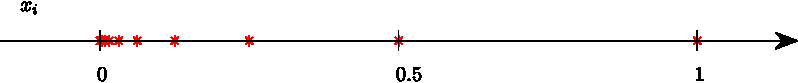
\includegraphics[width=0.8\columnwidth]{figures/graded_mesh.eps}
	\caption{ Example of a geometrically graded mesh using grading constant $0.5$
	In the listing \ref{code:cgauleg} the grading constant is set in line \texttt{6}.}
	\label{fig:graded_mesh}
\end{figure}
An example for a geometrically graded mesh can be seen in figure \ref{fig:graded_mesh}.
Each of the generated intervals is endowed with it's own Gauss-Legendre quadrature rule.
The details of the algorithm are shown in the listing \ref{code:cgauleg}.
\lstinputlisting[language=C++, caption={The function \texttt{cgauleg\_redux} takes the order and tolerance for which to compute the individual Gauss-Legendre quadrature rules and returns a composite Gauss-Legendre quadrature rule for the interval $\protect{[0,1]}$.}, label={code:cgauleg}]{code/cgauleg_redux.cpp}
It can be seen in lines \texttt{6} through \texttt{9} that the first interval is set to be of length $1-(\sqrt{2}-1)^2$.
At each step the interval is shifted towards zero by replacing the right boundary of the current interval with the left one and multiplying the left boundary by $(\sqrt{2}-1)^2$ as shown in line \texttt{29} and \texttt{30}.
In our algorithm while the length of the interval gets reduced the order of the Gauss-Legendre quadrature rule computed on that interval is reduced as well.
This is done by reducing the counter \texttt{qq} at each iteration in line \texttt{27} that is then used in line \texttt{19} to set the order of the computed Gauss-Legendre quadrature rule.
This reduces computational cost and we could verify that we don't loose any precision.

The algorithm in listing \ref{code:cgauleg} generates a one dimensional quadrature rule.
However we are computing double integrals in formula \ref{eq:param_int}.
This can be done by generating a tensor product quadrature rule as shown in listing \ref{code:tensor_prod}.
\lstinputlisting[language=C++, caption={The points and weights of the tensor product quadrature rule are computed by looping over a composite Gauss-Legendre quadrature rule for each dimension.}, label={code:tensor_prod}]{code/tensor_prod.cpp} 
In the next section we will talk about projecting BIOs computed using the standard basis for the spaces \ref{eq:FEMsp1} and \ref{eq:FEMsp2} to BIOs computed with orthonormal basis functions.

\section{Switching to Othonormal Basis} \label{sec:po}
Once the discretized operators have been computed using the Galerkin discretization (\ref{gbem}) and the composite Gauss-Legendre quadrature rule (\ref{cg}) it is helpful to project them using orthonormal basis functions. 
This has the advantage that the euclidean inner product on the expansion coefficients with respect to the basis becomes equivalent to the common inner product on $L^2(\Gamma)$ which allows for computing the singular values that converge towards the ones of the actual operators.
The technique used here to project the operators was described in \cite{LAN16}.
We will refer to the $L^2(\Gamma)$ inner product by $(\cdot,\cdot)$ from here on.
To compute an orthonormal basis (ONB) $(q_1,...,q_N)$ from an arbitrary basis $(b_1,...,b_N)$ we introduce the transformation matrix $\mathbf{T}$ which defines the ONB by:
\begin{equation}
	q_i  = \sum_{l=1}^N (\mathbf{T})_{il}b_l.	
\end{equation}
In order to satisfy the orthonormality condition $(q_i,q_j) = \delta_{ij}$ we require:
\begin{equation}
	\sum_l\sum_m(\mathbf{T})_{il}(\mathbf{T})_{jm}(b_l,b_m) = \delta_{ij}. \label{onbt1}
\end{equation}
In matrix form \ref{onbt1} can be written as $\mathbf{T}\mathbf{M}\mathbf{T}^T=\mathbf{I}$ with $\mathbf{M}=[(b_l,b_m)]_{l,m\geq1}^N$.
Using the decompositions:
\begin{align}
	\text{Cholesky}:& &\mathbf{M} &= \mathbf{LL}^T,& &\mathbf{L} \text{ lower left triangular }\\
	\text{QR}:& &\mathbf{L} &= \mathbf{QR},& &\mathbf{Q}\text{ orthogonal }
\end{align}
we can see that $\mathbf{T}:= \mathbf{R}^{-1}\mathbf{Q}^T$ satisfies \ref{onbt1}.
Therefore we can use $\mathbf{T}$ on our computed operator matrices to project them onto FEM-spaces with an orthonormal basis.
If we wanted to project an approximated BIO $\mathbf{A}_N$ computed with the basis $(b_1,...,b_N)$ onto the FEM-space spanned by $(q_1,...,q_N)$ we would compute $\mathbf{\tilde{A}}_N=\mathbf{TAT}^T$.
The singular values of the matrix $\mathbf{\tilde{A}}_N$ will then converge towards the singular values of the BIO we were approximating with $\mathbf{A}_N$.
In the next section we compute the derivatives of singular values of operators.
The technique holds for operators gained by the projection technique described here since it holds for arbitrary complex matrices.

\section{Computing the Derivative of Singular Values} \label{sec:svder}
In this section we will consider $\mathbf{A}(t) \in \mathbb{C}^{n \times n}$ to be an arbitrary complex matrix depending on a parameter $t$.
The singular value decomposition (SVD) of the matrix  $\mathbf{A}$ is given by:
\begin{equation}
	\mathbf{A} = \mathbf{U}\boldsymbol{\Lambda}\mathbf{V}^* \label{svd}
\end{equation}
where $\mathbf{U}$ is a unitary matrix, $\boldsymbol{\Lambda}$ is a diagonal matrix and $\mathbf{V}^*$ is the hermitian of a unitary matrix. 
Any matrix has a SVD as is shown in it's historic context in \cite{Stewart92onthe}.
We will compute the first and second derivative of $\mathbf{A}$'s singular values with respect to $t$ using the Jordan-Wielandt approach.
The Jordan-Wielandt approach relies on the fact that the Wielandt matrix of $\mathbf{A}$ defined as
\begin{equation}
	\mathbf{W}(t) := 
	\begin{bmatrix}
		0 & \mathbf{A}(t) \\
		\mathbf{A}^*(t) & 0 \\
	\end{bmatrix}
	\in \mathbb{C}^{2n \times 2n}
\end{equation}
has eigenvalues equal to $\pm$ the singular values of $\mathbf{A}(t)$.
We will prove this.
\begin{theorem}\label{thm:svd}
	The Wielandt matrix of an arbitrary complex matrix $\mathbf{A}$ has eigenvalues that are equal to $\pm$ the singular values of $\mathbf{A}$.
\end{theorem}
\begin{proof}
	Using the SVD from equation \ref{svd} we can rewrite the Wielandt matrix $\mathbf{W}$ as follows:
	\begin{align}
		\mathbf{W} := 
		\begin{bmatrix}
			0 & \mathbf{A} \\
			\mathbf{A}^* & 0 \\
		\end{bmatrix} &=
		\begin{bmatrix}
			0 & \mathbf{U}\boldsymbol{\Lambda}\mathbf{V}^* \\
			\mathbf{V}\boldsymbol{\Lambda}\mathbf{U}^*& 0 \\
		\end{bmatrix}\\ 
		&= \frac{1}{2}
		\begin{bmatrix}
			0 & 2\mathbf{U}\boldsymbol{\Lambda}\mathbf{V}^* \\
			2\mathbf{V}\boldsymbol{\Lambda}\mathbf{U}^*& 0 \\
		\end{bmatrix}\\ 
		&= \frac{1}{2}
		\begin{bmatrix}
			\mathbf{U}\boldsymbol{\Lambda} & -\mathbf{U}\boldsymbol{\Lambda} \\
			\mathbf{V}\boldsymbol{\Lambda}& \mathbf{V}\boldsymbol{\Lambda} \\
		\end{bmatrix} 
		\begin{bmatrix}
			\mathbf{U^*} & \mathbf{V^*} \\
			\mathbf{U^*} & -\mathbf{V^*} \\
		\end{bmatrix}\\ 
		& = \frac{1}{2}
		\begin{bmatrix}
			\mathbf{U} & \mathbf{U} \\
			\mathbf{V} & -\mathbf{V} \\
		\end{bmatrix}
		\begin{bmatrix}
			\boldsymbol{\Lambda} & 0 \\
			0 & -\boldsymbol{\Lambda} \\
		\end{bmatrix}
		\begin{bmatrix}
			\mathbf{U^*} & \mathbf{V^*} \\
			\mathbf{U^*} & -\mathbf{V^*} \\
		\end{bmatrix}. \label{evd}
	\end{align}
	Due to $\mathbf{U}$ and $\mathbf{V}$ being unitary the matrix 
	$\frac{1}{\sqrt{2}}
	\begin{bmatrix}
		\mathbf{U} & \mathbf{U} \\
		\mathbf{V} & \mathbf{-V}
	\end{bmatrix}$
	is unitary as well.
	This means we have retrieved the eigenvalue decomposition of $\mathbf{W}$ in equation \ref{evd} and the eigenvalues are indeed $\pm$ the singular values of $\mathbf{A}$.

\end{proof}
Using this result we will proceed by showing how to compute the first and second derivative of the eigenvalues of the Wielandt matrix $\mathbf{W}(t)$.
\subsection{Compute First Derivative}
In this section $(\cdot,\cdot)$ refers to the euclidean inner product on the appropriate space.
Theorem \ref{thm:svd} implies that there exists an eigenvector $ [\mathbf{x}_1(k), \mathbf{x}_2(k)]^T \in \mathbb{C}^{2n} \setminus \{0\}$ so that:
\begin{equation}
	\left(\mathbf{W}(t)
		\begin{bmatrix}
			\mathbf{x}_1 \\ \mathbf{x}_2
		\end{bmatrix}
		,
		\begin{bmatrix}
			\mathbf{v}_1 \\ \mathbf{v}_2
		\end{bmatrix}
		\right) = \lambda(t) \left(
		\begin{bmatrix}
			\mathbf{x}_1 \\ \mathbf{x}_2
		\end{bmatrix}
		,
		\begin{bmatrix}
			\mathbf{v}_1 \\ \mathbf{v}_2
		\end{bmatrix}
	\right) \quad \forall 
	\begin{bmatrix}
		\mathbf{v}_1 \\ \mathbf{v}_2
	\end{bmatrix}
	\in \mathbb{C}^{2n}.
\end{equation}
This is a generalized eigenvalue problem.
In terms of $\mathbf{A}(t)$ it gives us:
\begin{align}
	(\mathbf{A}(t)\mathbf{x}_2, \mathbf{v}_1) + (\mathbf{x}_1(t),\mathbf{A}(t)\mathbf{v}_2) =\lambda(t)[(\mathbf{x}_1(t),\mathbf{v}_1) + (\mathbf{x}_2(t), \mathbf{v}_2)]
	\quad \forall \mathbf{v}_1, \mathbf{v}_2 \in \mathbb{C}^n.  \label{svder1}
\end{align}
Performing implicit differentiation in $t$ gives:
\begin{align}
	\begin{split}
		&(\mathbf{A}'(t)\mathbf{x}_2, \mathbf{v}_1) + (\mathbf{A}(t)\mathbf{x}'_2, \mathbf{v}_1) + (\mathbf{x}'_1(t),\mathbf{A}(t)\mathbf{v}_2) + (\mathbf{x}_1(t),\mathbf{A}'(t)\mathbf{v}_2) 
		\\ = &\lambda'(t)[(\mathbf{x}_1(t),\mathbf{v}_1) + (\mathbf{x}_2(t), \mathbf{v}_2)] + \lambda(t)[(\mathbf{x}'_1(t),\mathbf{v}_1) + (\mathbf{x}'_2(t), \mathbf{v}_2)]
		\quad \forall \mathbf{v}_1, \mathbf{v}_2 \in \mathbb{C}^n.
	\end{split} \label{svder2}
\end{align}
Substituting $\mathbf{v}_1$, $\mathbf{v}_2$ for $\mathbf{x}_1'(k)$, $\mathbf{x}_2'(k)$ in \ref{svder1} and for $\mathbf{x}_1(k)$, $\mathbf{x}_2(k)$ in \ref{svder2} we can then subtract the complex conjugate of \ref{svder1} from \ref{svder2} leaving us with:
\begin{align}
	(\mathbf{A}'(k)\mathbf{x}_2, \mathbf{x}_1) + (\mathbf{x}_1,\mathbf{A}'(k)\mathbf{x}_2) =
	\lambda'(k) 
	\label{svder3}
\end{align}
where we assumed that $\mathbf{x}_1$ and $\mathbf{x}_2$ have already been normalized so that $||\mathbf{x}_1(k)||^2 + ||\mathbf{x}_2(k)||^2 = 1$.
Here and for the rest of this chapter $||\cdot||$ is the norm induced by $(\cdot,\cdot)$.
To compute the derivative of the singular values of $\mathbf{A}$ is now simply a matter of computing the operator derivative in $t$, finding the eigenvectors of the Wielandt matrix and plugging these quantities into \ref{svder3}.
This gives us the eigenvalues of $\mathbf{W}$ which are, as shown in theorem \ref{thm:svd}, $\pm$ the singular values of $\mathbf{A}$.
Of course this can be done with the discretized operators computed by Galerkin BEM.
It is especially straight forward when using the projected operators according to section \ref{sec:po} since then the inner product on the FEM-spaces becomes equivalent to the euclidean one used here.
In this section we are actually not making any assumptions that wouldn't hold for an arbitrary operator.
Therefore this method of computing the derivative of singular values actually holds for any operator with a SVD and not just complex matrices.
In the next section we will compute the second derivative of the singular values of the matrix $\mathbf{A}$.

\subsection{Compute Second Derivative}
Using the theorem \ref{thm:svd} once more we will compute the second derivative of the singular values of $\mathbf{A}$ by computing the second derivative of the eigenvalues of the Wielandt matrix $\mathbf{W}$.
The algorithm described here was taken from \cite{doi:10.1002/nme.1620260202}.
We start out with the $t$-dependent eigenvalue problem for the Wielandt matrix and it's derivative:
\begin{align}
	\mathbf{W}(t)\mathbf{u}(t) &= \lambda(t)\mathbf{u}(t) \\
	\mathbf{W}'(t)\mathbf{u}(t) +
	\mathbf{W}(t)\mathbf{u}'(t) &=
	\lambda'(t)\mathbf{u}(t) +
	\lambda(t)\mathbf{u}(t)' \label{eq:evder}
\end{align}
where $\mathbf{u}$ is an eigenvector of $\mathbf{W}$ and $\lambda$ is the corresponding eigenvalue.
In order to uniquely define the eigenvector $\mathbf{u}$ we will define the normalization condition:
\begin{align}
	\mathbf{u}_m(t) = 1. \label{eq:norm_cond}
\end{align}
The subscript $m$ denotes the $m$-th entry of the vector $\mathbf{u}$.
Choosing this normalization condition instead of the more stable $||u|| = 1$ is essential and will be used later on for the derivation of the algorithm.
In order to regain some stability we choose $m$ so that:
\begin{equation}
	\max_{i \in \{1,...,2n\}} \mathbf{u}_i(t) = \mathbf{u}_m(t).
\end{equation}
We will drop the explicit time dependence from here out.
The equation \ref{eq:evder} can be written in block matrix form as follows:
\begin{align}
	\begin{bmatrix}
		\mathbf{W}-\lambda\mathbf{I} & -\mathbf{u}
	\end{bmatrix}
	\begin{bmatrix}
		\mathbf{u}' \\
		\lambda'
	\end{bmatrix} 
	= - \mathbf{W}'\mathbf{u}. \label{eq:evder_block}
\end{align}
Using the derivative of the normalization condition \ref{eq:norm_cond} we can rewrite equation \ref{eq:evder_block} as:
\begin{align}
	\mathbf{\tilde{W}} \mathbf{\tilde{u}}' = -\mathbf{W}\mathbf{u} \label{eq:firstder}
\end{align}
with the definitions:
\begin{align}
	\mathbf{\tilde{W}} &:= 
	\begin{bmatrix}
		\mathbf{W}-\lambda\mathbf{I}  -\mathbf{u}
	\end{bmatrix}
	_{\text{$m$-th column removed}} \\
	\mathbf{\tilde{u}} &:=  
	\begin{bmatrix}
		\mathbf{u} \\
		\lambda
	\end{bmatrix} 
	_{\text{$m$-th entry removed}}.
\end{align}
Using \ref{eq:firstder} we can compute the first derivative of the eigenvalues and eigenvectors of $\mathbf{W}$.
We will use these to compute the second derivatives.
This is done analogously as for the first derivatives by taking equation \ref{eq:evder}, computing it's derivative, and applying the normalization condition \ref{eq:norm_cond}.
The result is:
\begin{align}
	\mathbf{\tilde{W}} \mathbf{\tilde{u}}'' 
	= -\mathbf{W}''\mathbf{u} - 2(\mathbf{W}'-\lambda'\mathbf{I})\mathbf{u}'. \label{eq:final_res}
\end{align}
The equation \ref{eq:final_res} lets us compute the second derivative of an eigenvalue of $\mathbf{W}$ as the last entry of the vector $\mathbf{\tilde{u}}''$.
According to theorem \ref{thm:svd} this gives of the second derivatives of the singular values of $\mathbf{A}$.
In the next section we will describe the algorithms used to compute the minima in the singular values of $\mathbf{A}$ using the derivatives that we computed in this section.

\section{Root finding} \label{sec:roots}
The simplest method for root finding is bisection. 
However this method only has a linear convergence rate.
We will give a brief over view over the secant method, the Van Wijngaarden-Dekker-Brent method, and the Newton-Raphson method for root finding with higher convergence rates.

\subsection{Secant Method}
A simple method with superlinear convergence is the secant method. 
It takes the initial interval and assumes that the function in question is linear within.
Using this assumption the root is computed leading to the iteration step:
\begin{equation}
	x_n = x_{n-1} - f(x_{n-1})\frac{x_{n-1}-x_{n-2}}{f(x_{n-1})-f(x_{n-2})}
\end{equation}
The root found by this manner is than used as a new interval boundary.
The interval boundary that gets replaced is always the one that hasn't been updated the longest.
Given some constraints on the function $f$ the secant method's convergence rate is the positive solution of the equation:
\begin{align}
	x^2 -x -1 = 0
\end{align}
which is the "golden ratio" $x \approx 1.618$ \cite{doi:10.1002/9781118033128.ch3}.
However the secant method has some flaws as well.
First off it doesn't guarantee that the root that was bracketed in the beginning remains bracketed.
Furthermore there are certain pathological functions where bisection would actually lead to faster convergence.

\subsection{Van Wijngaarden-Dekker-Brent Method} 
A solution to these problems is the Van Wijngaarden-Dekker-Brent method. 
It switches between bracketing and the secant method depending on the convergence rate achieved by the secant method. 
Also instead of a linear fit between the two interval boundaries, an inverse quadratic fit based on three evaluation points $(a,f(a))$, $(b,f(b))$, $(c, f(c)$ is used which allows for a better approximation of the root at every step.
This gives us the following formula to approximate a root:
\begin{align}
	x  = \frac{f(a)f(b)c}{[f(c)-f(a)][f(c)-f(b)]} + \frac{f(b)f(c)a}{[f(a)-f(b)][f(a)-f(c)]} \\
	+\frac{f(c)f(a)b}{[f(b)-f(c)][f(b)-f(a)]} \label{eq:update_brent}
\end{align}
If the approximation $x$ turns out to lie outside of the current interval or if a division by zero would occur a bisection step is taken instead.
This keeps the potential root we are looking for bracketed.
Also if the boundaries don't collapse fast enough the update step \ref{eq:update_brent} is replaced by a bisection step as well.
With some conditions assumed upon $f$ the convergence rate is the positive solution of:
\begin{align}
	x^3 - x^2 - x -1 = 0.
\end{align}
This is approximately $x \approx 1.839$ \cite{brent1971algorithms}.
The implementation used in the code of this thesis is the one suggested in \cite{rf}
and can be checked in the listing \ref{code:zbrent}.

\subsection{Newton-Raphson Method}
For an even higher convergence rate there is the Newton-Raphson method.
The Newton-Raphson method relies on the Taylor expansion of the function $f$:
\begin{equation}
	f(x+\delta) \approx f(x) + f'(x)\delta + \frac{f''(x)}{2}\delta^2 + ...
\end{equation}
For a small $\delta$ and a well behaved function the terms beyond the linear one are negligible.
This gives the approximation of $\delta = -\frac{f(x)}{f'(x)}$ to find the point where $f(x+\delta)=0$.
For well behaved functions and near a minima the Newton-Raphson method converges quadratically \cite{traub2014analytic}
Since in our case $f$ is the first derivative of the singular value we need the singular values second derivative to compute the update of this algorithm.
This was obtained using the algorithms from \cite{doi:10.1002/nme.1620260202} that we described in section \ref{sec:svder}.
The algorithm to implement this root finding method was again taken from \cite{rf} and can also be checked in \ref{code:rtsafe}.

\subsection{Discontinuities in Derivatives of Singular Values}
When looking for minima in the map $\sigma_1(k)$ crossings of the different singular values have to be taken into account.
These lead to sign changes in the derivative which can be falsely identified as a root.
Examples of actual roots and false positives can be seen in the figure \ref{fig:crossings}.
The false positives are however easily discarded since the sign changes in these cases are accompanied by jumps.
Therefore simply evaluating the derivative at the found root after computation will tell if it is an actual minima or a crossing.
In the next section we will give an overview of the code structure inside the library that was developed in the course of this thesis.
\begin{figure} [H]
	\centering
	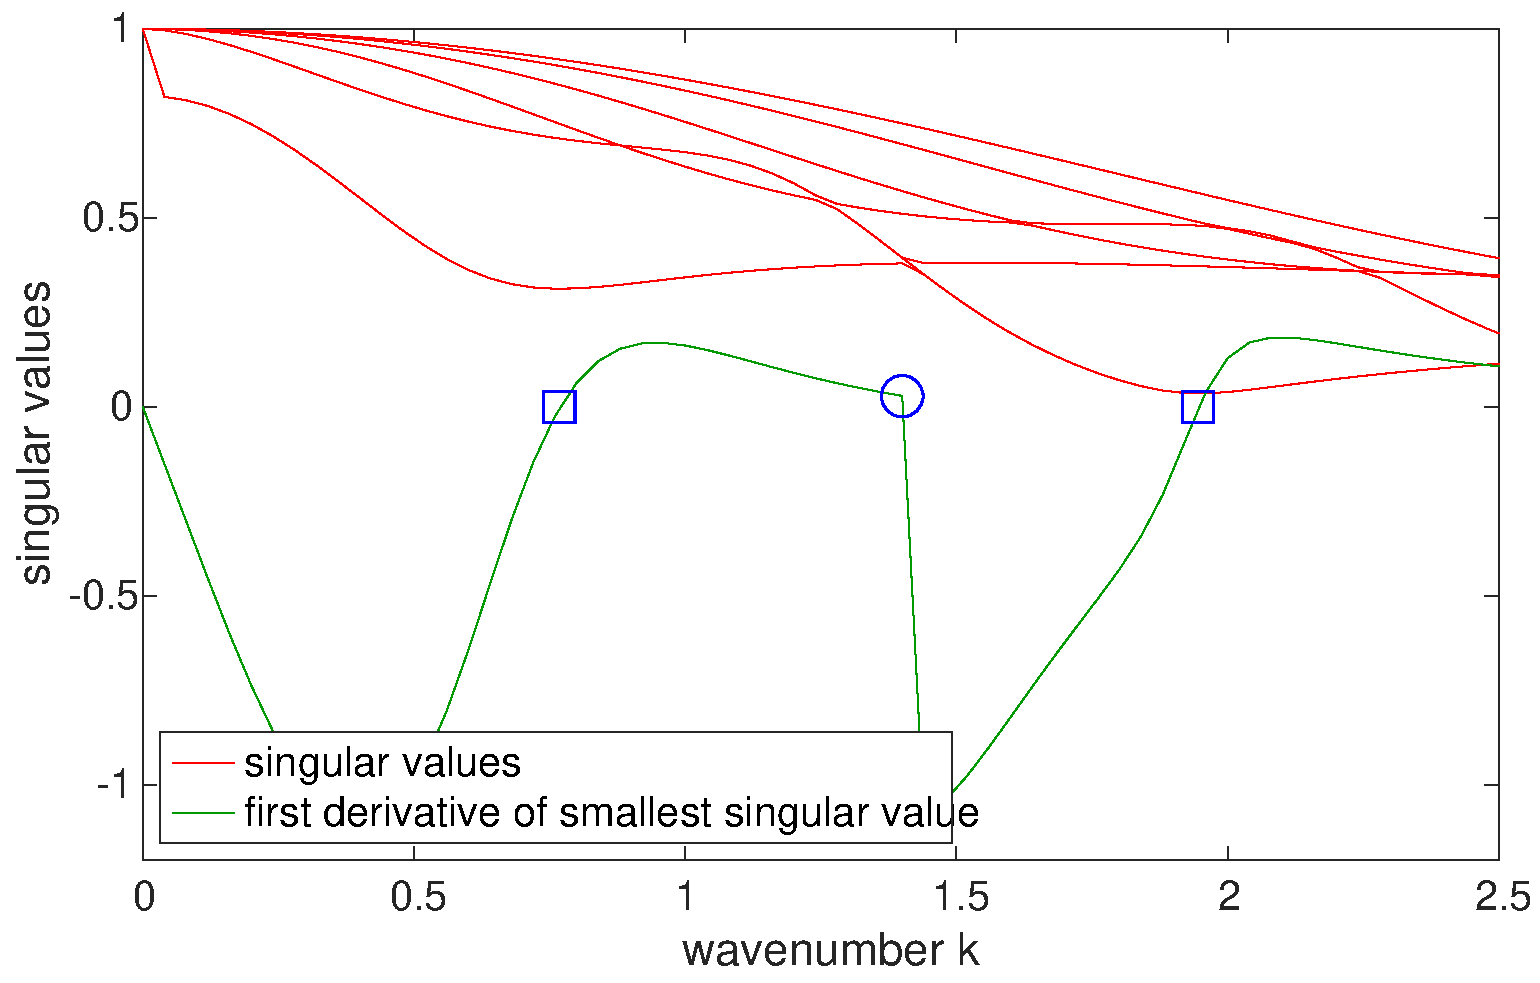
\includegraphics[width=\columnwidth]{figures/crossings.eps}
	\caption{ 
		$\textcolor{blue}\square$: Convergence points that are actual roots.
		$\textcolor{blue}\bigcirc$: Convergence point that is not a root.
		They can be differentiated by making an extra evaluation of the derivative after convergence.
	}
	\label{fig:crossings}
\end{figure}

\section{Code Structure}
The library developed in the course of this thesis was named HelmholtzTransmissionProblemBEM.
It consists of five main directories that can be seen in the directory tree \ref{dir:struct}.
The doxygen directory only contains the build configuration for the doxygen documentation.
The examples directory contains many \texttt{C++} driver scripts and Matlab plotting scripts that were used to generate the results in chapter \ref{chap:numres}.
Explanations on how to use these scripts can be found in the appendix \ref{chap:usage}.
The include directory contains all header files.
In the source directory the \texttt{C++} code for computing our BIOs defined in section \ref{sec:BIEs}, as well as their first and second derivative, can be found.
This directory also contains three subdirectories.
The parametrizations subdirectory containing classes to generate different parametrized boundaries, the quadrature subdirectory containing the functions that generate a standard and a composite Gauss-Legendre quadrature rule, and the utilities directory that contains many helpful functions such as functions for generating solutions of the form described in section \ref{sec:asc}, root finding or solvers for the BIEs from the section \ref{sec:BIEs}.
The test directory contains Google Test unit tests for each operator against a given correct computation as well as tests for the solutions generated by the functions placed in the utilities directory.
In the next chapter we will perform validation on our discretized BIOs and the algorithms for computing the derivatives of the singular values.
We will also compare the algorithms for root finding applied to our specific case.
\begin{figure}[H]
	\centering
	\framebox[\textwidth]{%
		\begin{minipage}{0.9\textwidth}
			\dirtree{%
				.1 HelmholtzTransmissionProblemBEM.
				.2 doxygen.
				.2 examples.
				.2 include.
				.2 source.
				.3 parametrizations.
				.3 quadrature.
				.3 utilities.
				.2 test.
			}
		\end{minipage}
	}
	\caption{The directory tree of the HelmholtzTransmissionProblemBEM library containing 5 directories and three subdirectories.} 
	\label{dir:struct}
\end{figure}

\chapter{Numerical Results} \label{chap:numres}
In order to verify the code that implements the algorithms from chapter \ref{code} we ran a series of tests that will be listed in this chapter. 
In the first section we will be validating the discretized operators.

\section{Validating Operators}
To validate the discretization of the boundary integral operators described in \ref{sec:BIEs} we ran some tests computing the baseline solution to an analytically solvable case of the Helmholtz transmission problem.
The general solutions are described in section \ref{sec:asc}.
As a baseline we used the series:
\begin{align}
	u_{res}(r,\phi) &=  T_0 H_0^{(1)}(k\sqrt{n_o}r) &\text{ in } \Omega_o \\
	u_{res}(r,\phi) &=  R_0 J_0(k\sqrt{n_i}r) &\text{ in } \Omega_i \\
	u_{inc}(r,\phi) &=  J_0(k\sqrt{n_o}r) &\text{ in } \mathbb{R}^2
\end{align}
with $\Omega_i=B_{1/4}(0)$, $n_o=1$, $n_i=5$, and $k=1$.
This will be the baseline for the rest of this chapter.
The functions $H_0^{(1)}$ and $J_0$ refer to the Hankel function of the first kind of $0$-th order and the Bessel function of $0$-th order respectively. 
\subsection{Determining Optimal Order of Gauss-Legendre Rule}
We ran our baseline model problem for different orders of the Gauss-Legendre quadrature rule used to compute the matrix entries of our approximated BIOs.
For panels that are disjoint a standard Gauss-Legendre quadrature rule was used.
Here the order just refers the order of the quadrature rule.
For adjacent and coinciding panels the composite Gauss-Legendre quadrature rule as described in section \ref{cg} was used.
Here the order refers to the order used on the first interval on which the Gauss-Legendre quadrature rule gets computed. 
The results of the tests can be seen in figure \ref{fig:order}.
\begin{figure} [!ht]
	\centering
	\includegraphics[width=\columnwidth]{figures/order.eps}
	\caption{ By $\tilde{u}$ and $u_h$ we refer to the known solution projected on to the FEM-spaces and the computed solution respectively.
		The norm $||\tilde{u}-u_h||_{L^2(\Gamma)}$ is equivalent to the norm induced by the euclidean inner product of the difference between the interpolation coefficients of $\tilde{u}$ and $u_h$ in the FEM-spaces once these have been projected according to section \ref{sec:po}.
		We will keep these notations throughout the rest of this thesis.
	}
	\label{fig:order}
\end{figure}
We can see that up to $order=11$ the convergence is stable. 
After this point the convergence breaks down on finer meshes.
This is most likely due to the quadrature rule evaluating the kernel in the integrals too closely to the singularities.
Due to these results we will be setting the $order$ to $11$ for the rest of the experiments.
In the next sections we will see how convergence varies due to changes in parameters such as wavenumber, refraction index and series expansion of the known solution.

\subsection{Varying Wavenumber}
Here we keep our baseline problem and vary only the parameter $k$.
The results can be seen in \ref{fig:wavenumber}.
\begin{figure} [!ht]
	\centering
	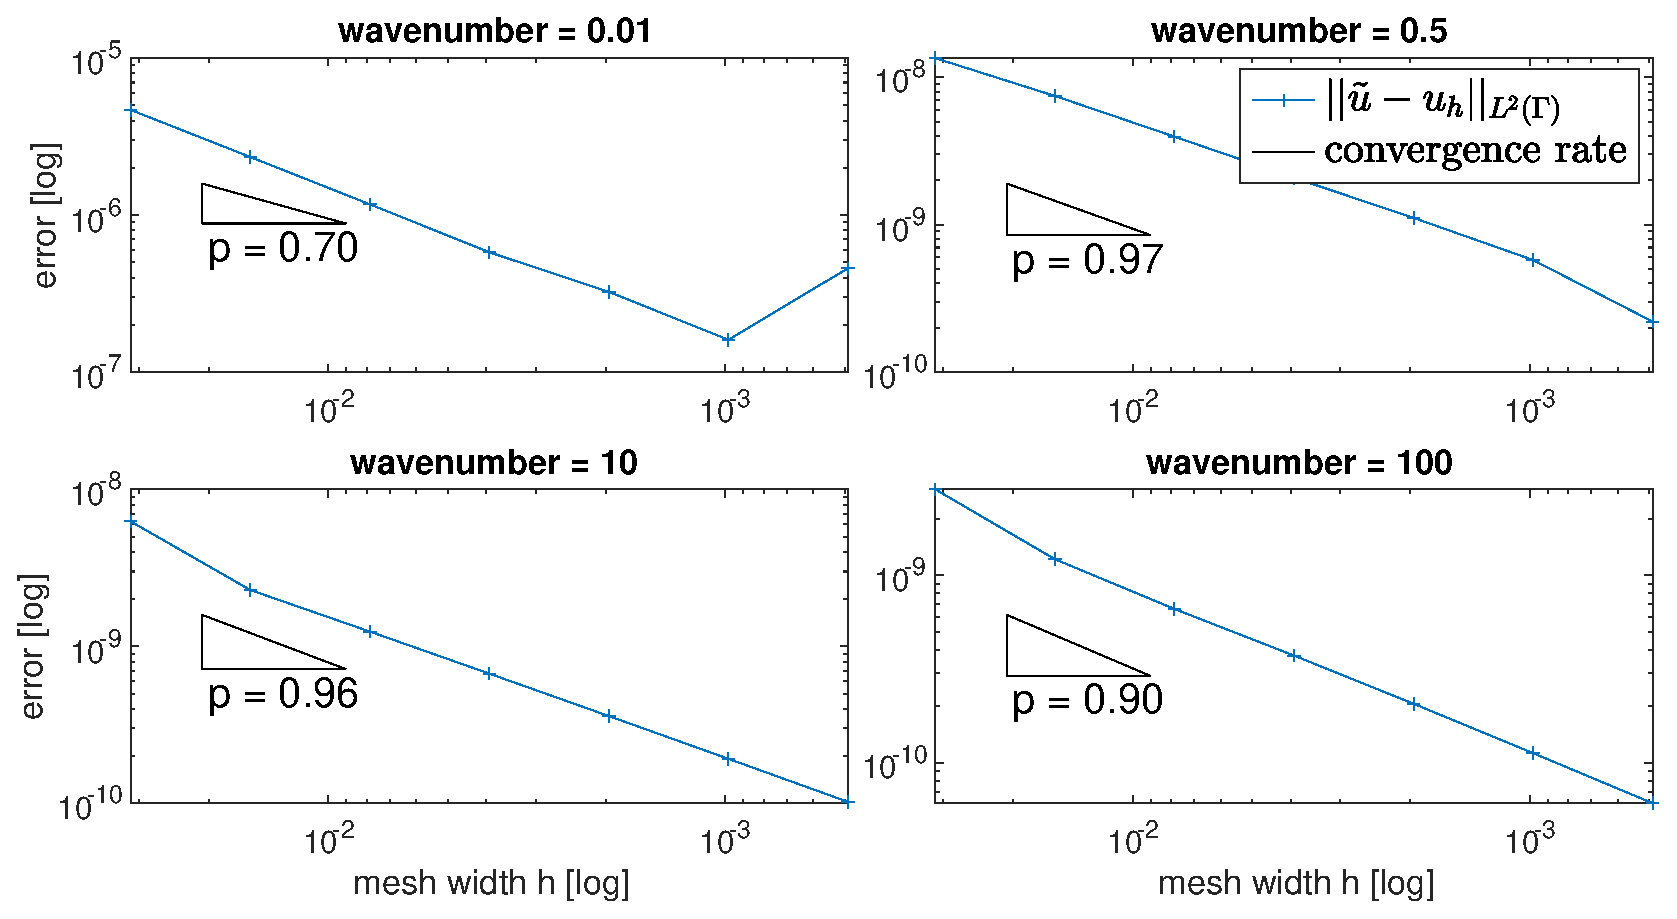
\includegraphics[width=\columnwidth]{figures/wavenumber.eps}
	\caption{ These figures show some examples of the convergence rate over different wavenumbers.
	The convergence rate is stable except for the edge case $k=0.01$}
	\label{fig:wavenumber}
\end{figure}
It can be seen that the convergence rate remains relatively stable except for in the case where $k=0.01$.
This is due to the fact that for small $k$'s the argument in the kernels of the integrals become smaller for the same evaluation points along the boundary.
Therefore we are again evaluating the kernels in the integrals too closely to the singularities for very fine meshes as we did when using quadrature rules of too high orders.
This is difficult to avoid since doing so indiscriminately could lead to loosing precision in stable cases.
%cases where the convergence rate is stable at the moment.
\subsection{Varying Refraction Index}
For these results we again kept the baseline problem but varied the refraction index $n_i$.
The results are plotted in figure \ref{fig:refraction} on the following page.
\begin{figure} [!ht]
	\centering
	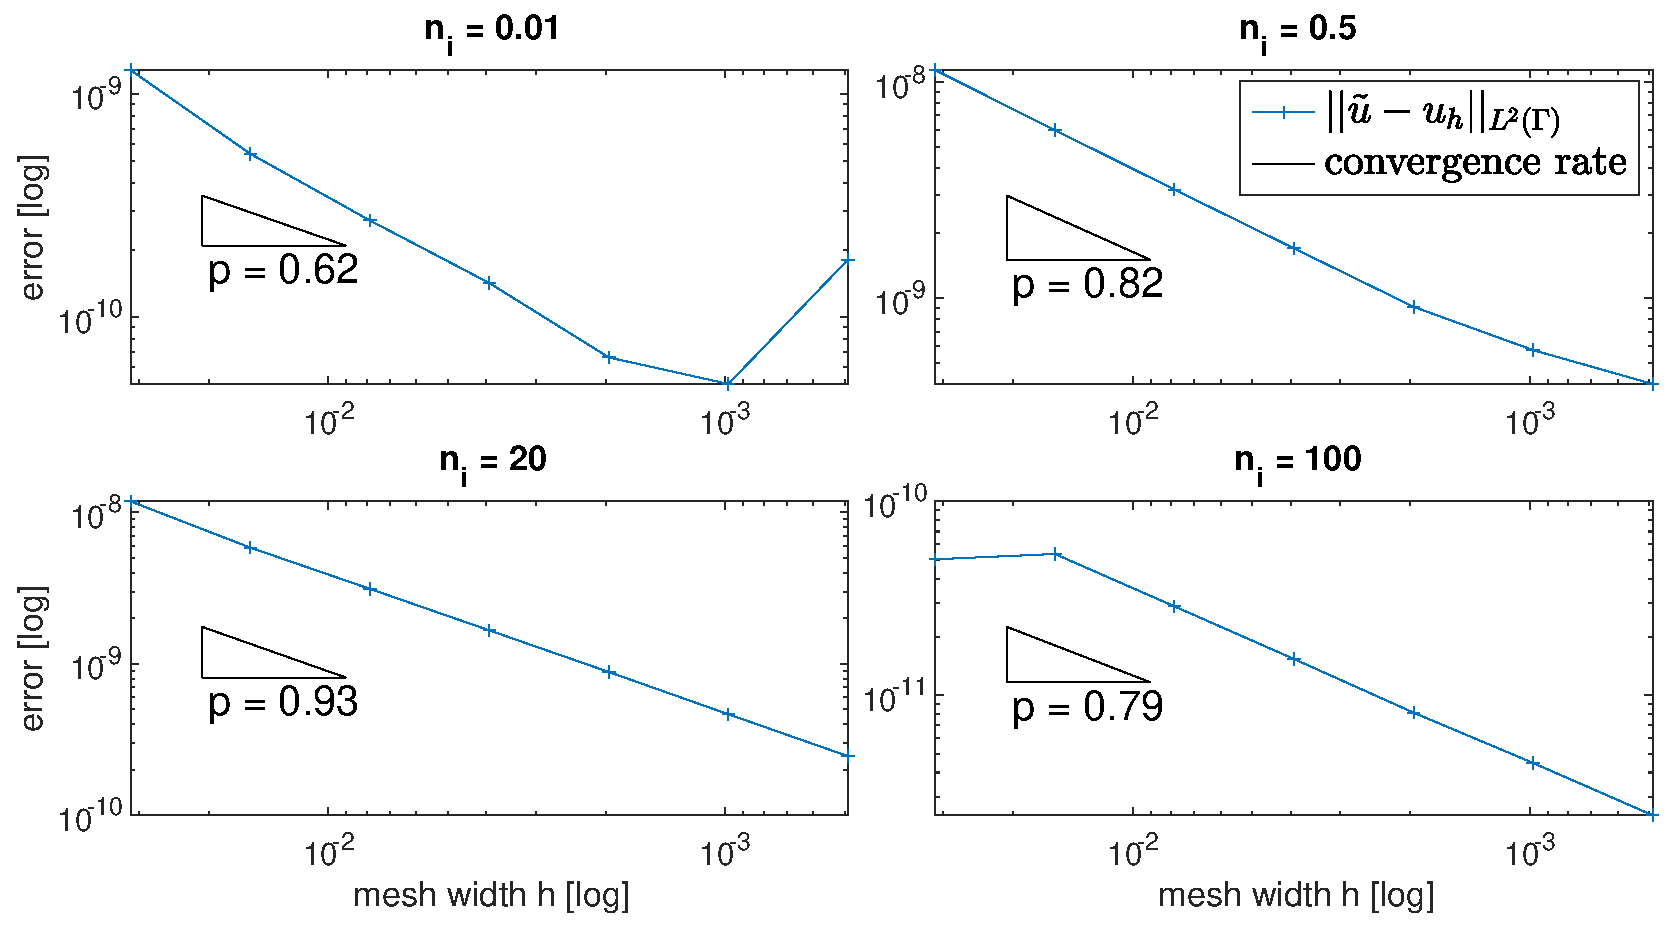
\includegraphics[width=\columnwidth]{figures/refraction.eps}
	\caption{
		Here we plotted the convergence rates for different refraction indices.
	As with varying the wavenumber, the convergence is mostly stable except for edge cases.}
	\label{fig:refraction}
\end{figure}
When varying the refraction index we can see that for small indices and fine grids the convergence collapses as well as for large indices and coarse grids.
This is because the larger the refraction index becomes, the more the kernels of the BIOs will vary along the same panel.
So for large indices having a low order quadrature rule will not be enough to capture this fluctuation.
For small indices however the problem remains to be too close evaluation of the kernels around the singularities as was the case in the previous two sections.
%\begin{figure} [H]
%	\centering
%	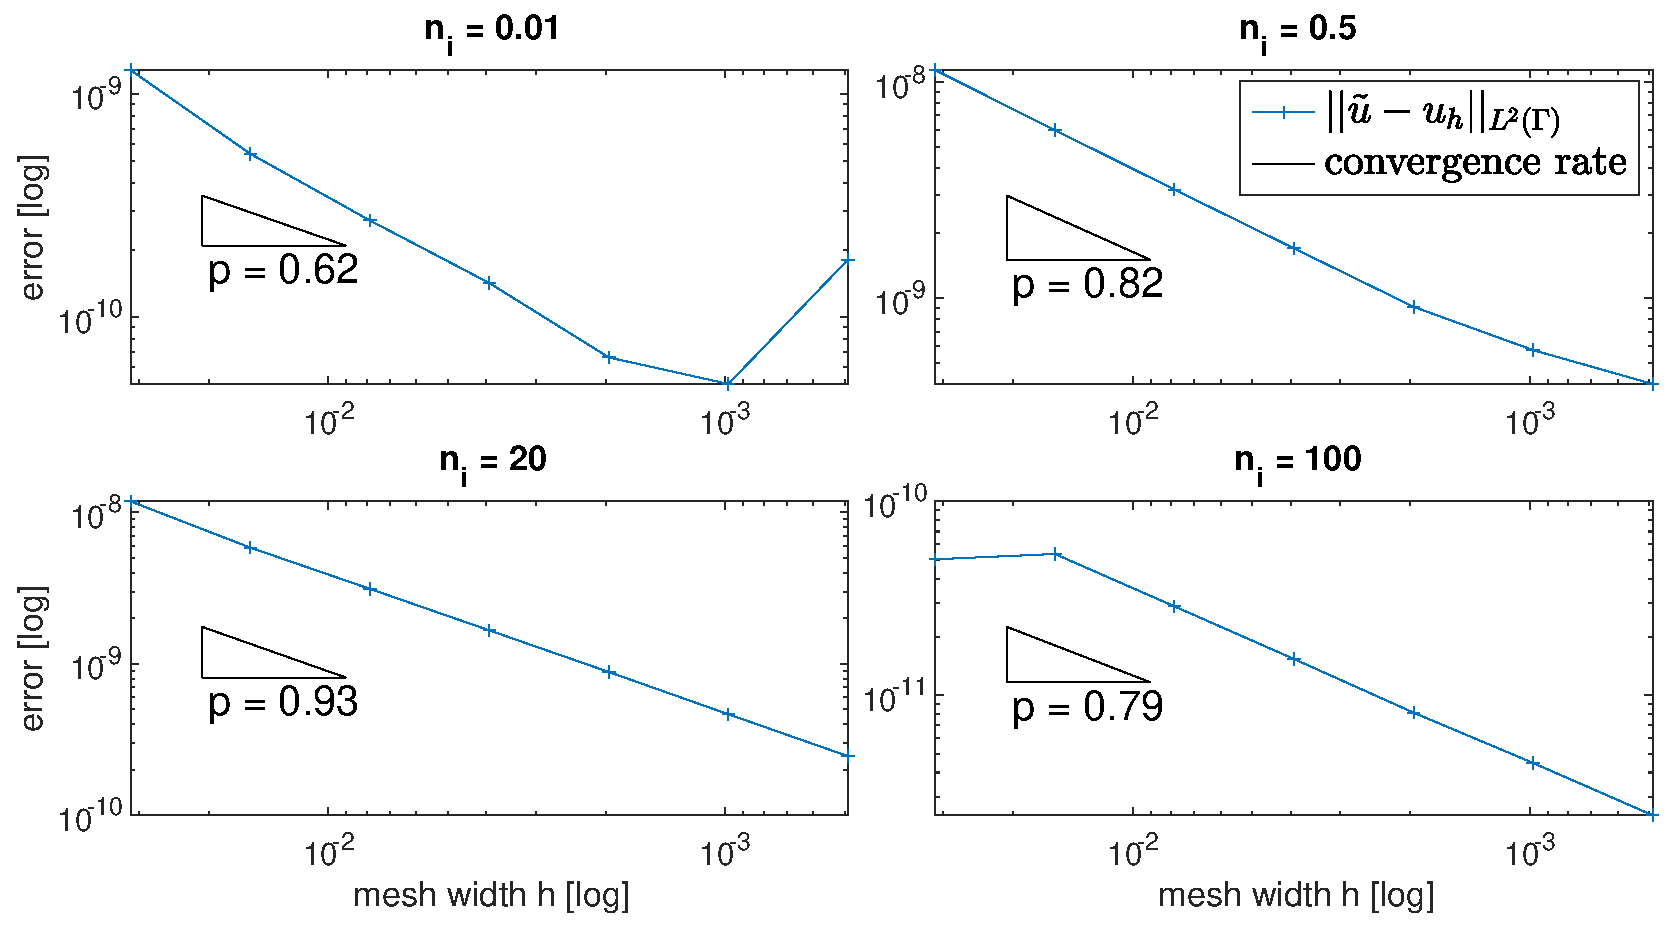
\includegraphics[trim=0 270 0 21, clip,width=\columnwidth]{figures/refraction.eps}
%	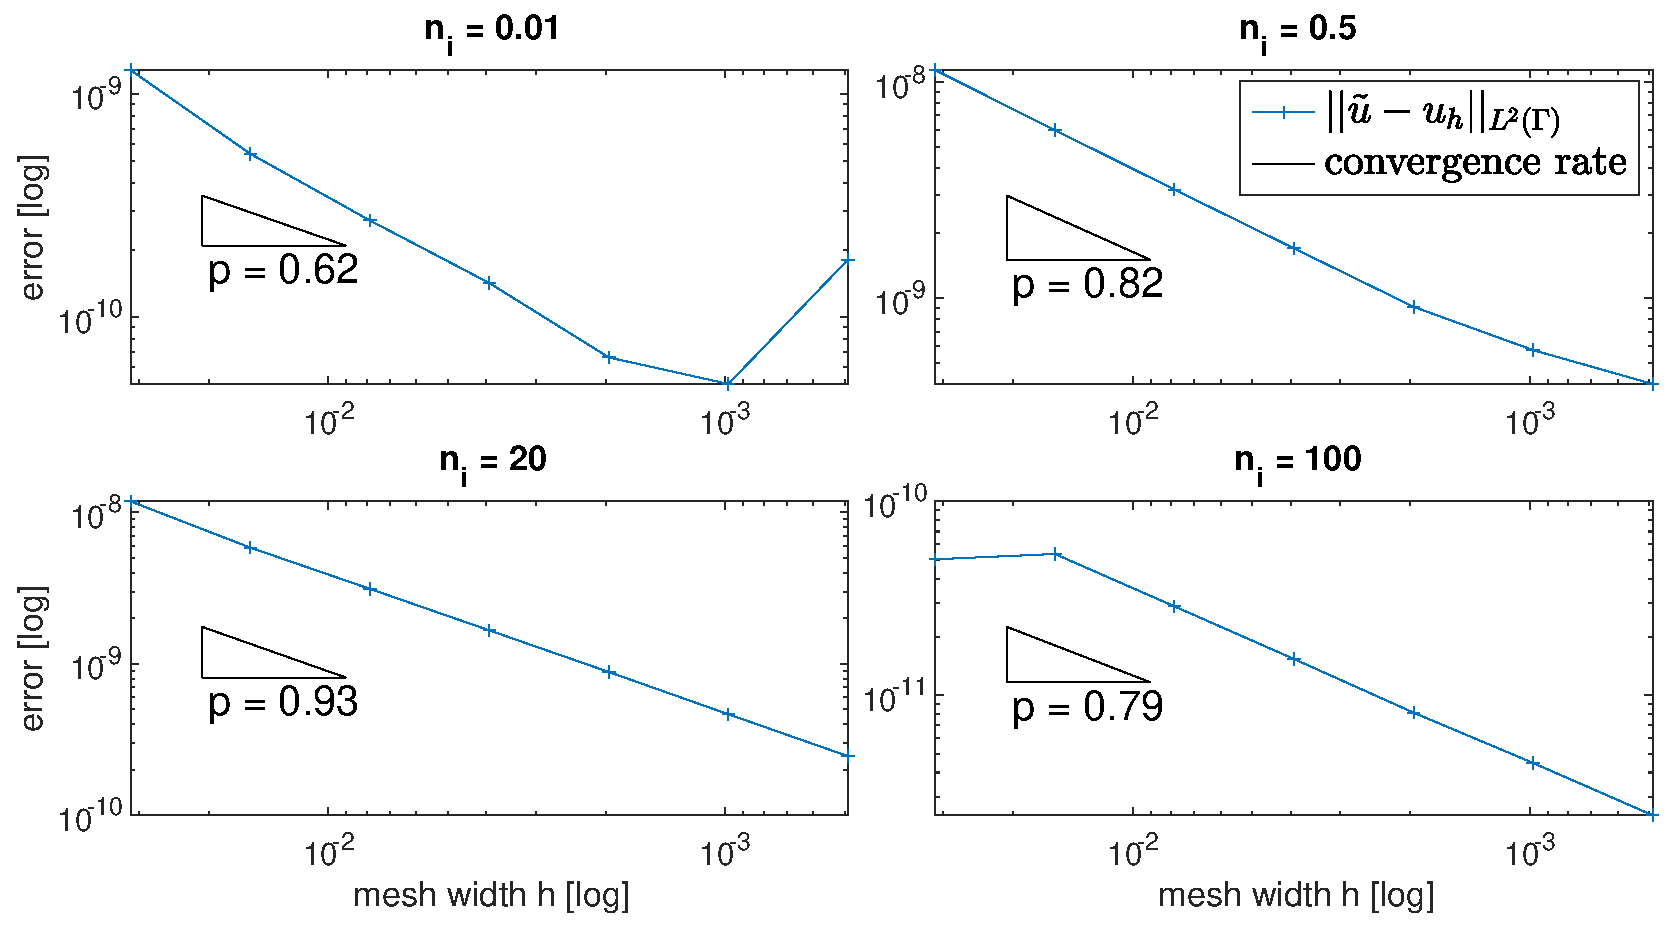
\includegraphics[trim=0 16 0 488, clip,width=\columnwidth]{figures/refraction.eps}
%\end{figure}
%\begin{figure} [H]
%	\centering
%	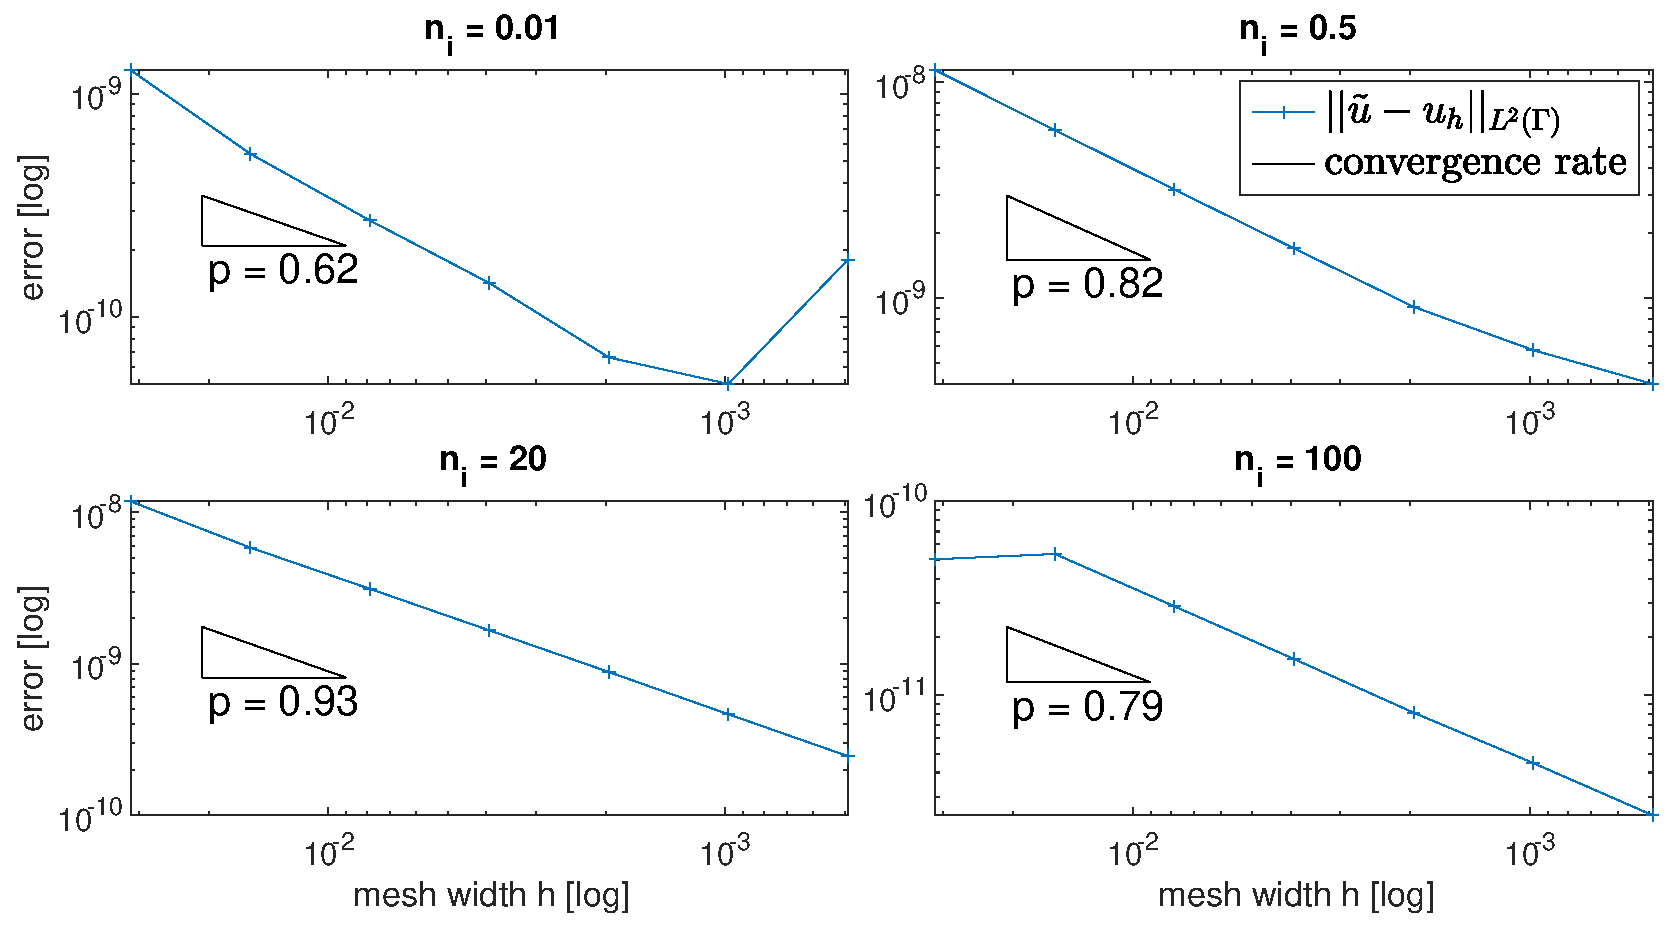
\includegraphics[trim=0 16 0 252, clip,width=\columnwidth]{figures/refraction.eps}
%	\caption{
%		Here we plotted the convergence rates for different refraction indices.
%	As with varying the wavenumber, the convergence is mostly stable except for edge cases.}
%	\label{fig:refraction}
%\end{figure}

\subsection{Varying Incoming Wave}
What we are varying here is the series expansion of the incoming wave and the expected solution.
The series expansion used is stated in section \ref{sec:asc}.
The results for different numbers of non-zero coefficients are plotted in the figure \ref{fig:solutions}.
\begin{figure} [!ht]
	\centering
	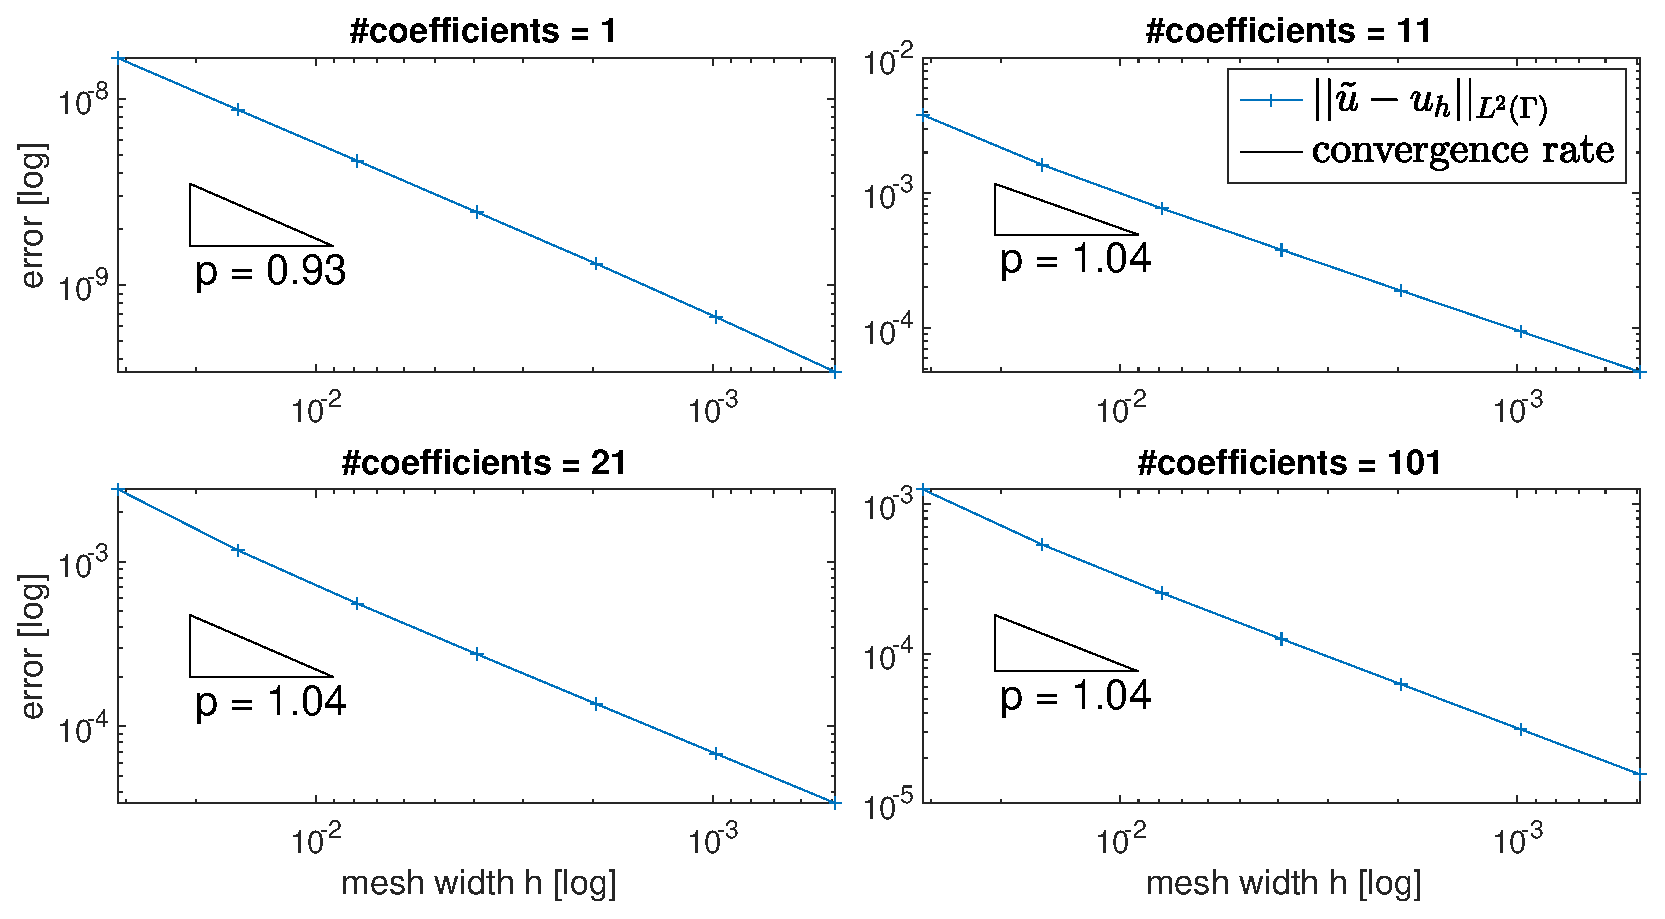
\includegraphics[width=\columnwidth]{figures/solutions.eps}
	\caption{ Here we plotted the convergence rates for different incoming waves.
	The convergence rate stays stable in all cases that we observed.}
	\label{fig:solutions}
\end{figure}
Although the convergence remains stable the magnitude of the error varies.
This is due to the solutions being of different orders of magnitude themselves causing the absolute error to vary.
As we can see there is no breakdown in convergence here.
This leads us to believe that the convergence is independent of the solution, at least if it is of the form as stated in section \ref{sec:asc}.

The results of the previous sections showed us that our discretized operators are correct for most reasonable combinations of meshes and parameters.
The results from \cite{svdap} tell us that the singular values of the discretized operators converge towards the ones of the operator itself.
Using this fact together with our validation we can now assume that the singular values of the discretized operators we compute for the Helmholtz transmission problem approximate those of the actual operators that model this problem.
To see if we can get some evidence of this we will be looking at some computed singular values for different mesh sizes.

\section{Validating Singular Values} \label{sec:valsv}
To see if the change in our singular values reduced as we computed them using operators approximated on finer meshes we compared the smallest ten singular values of our baseline problem while decreasing the grid size of our mesh.
The results can be seen in the table \ref{tbl:sv}
\begin{table}[h!]
	\centering
	\begin{tabular}{ |c|c|c|c|c|c| } 
		\hline
		h & 0.0157 & 0.0079 & 0.0039 & 0.0020 & 0.0010 \\ 
		\hline
		$\bigtriangleup$ & 0.0040 & 0.0021 & 0.0011 & 0.0005 & 0.0002 \\ 
		\hline
	\end{tabular}
	\caption{Change in singular values against change in grid size.}
	\label{tbl:sv}
\end{table}
Here $h$ refers to the grid size on the finer mesh on which we are comparing the singular values up to 4 digits after the decimal point.
$\bigtriangleup$ refers to the difference between the singular values computed on the mesh with grid size $h$ to the ones computed on the mesh with grid size $h/2$.
It can be seen that the difference goes towards $0$ in the order of $h$.
This is reflected in figure \ref{fig:SVs_circle} where the 20 smallest singular values are plotted.
\begin{figure} [!ht]
	\centering
	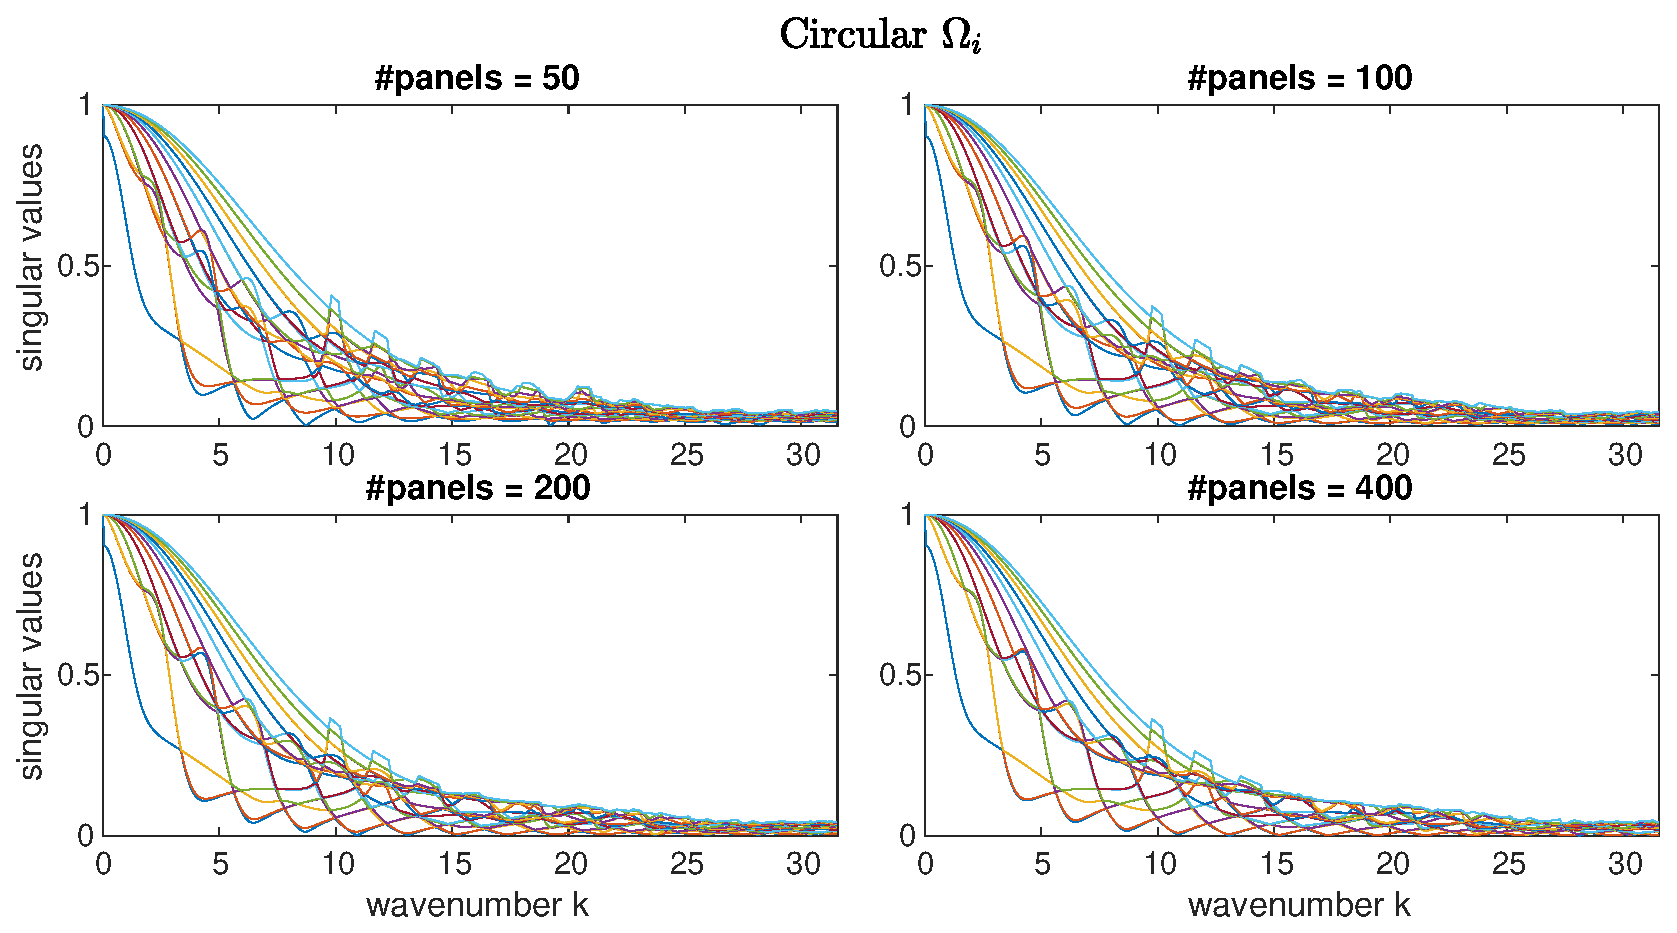
\includegraphics[width=\columnwidth]{figures/SVs_circle.eps}
	\caption{ The singular values on the circle can be seen to converge. 
	Most importantly this is the case for the smallest singular value which we will be using later on to determine resonances.}
	\label{fig:SVs_circle}
\end{figure}
The same can be said when switching our domain in our baseline problem from a circle to a square.
The results can be seen in figure \ref{fig:SVs_square}.
\begin{figure} [!ht]
	\centering
	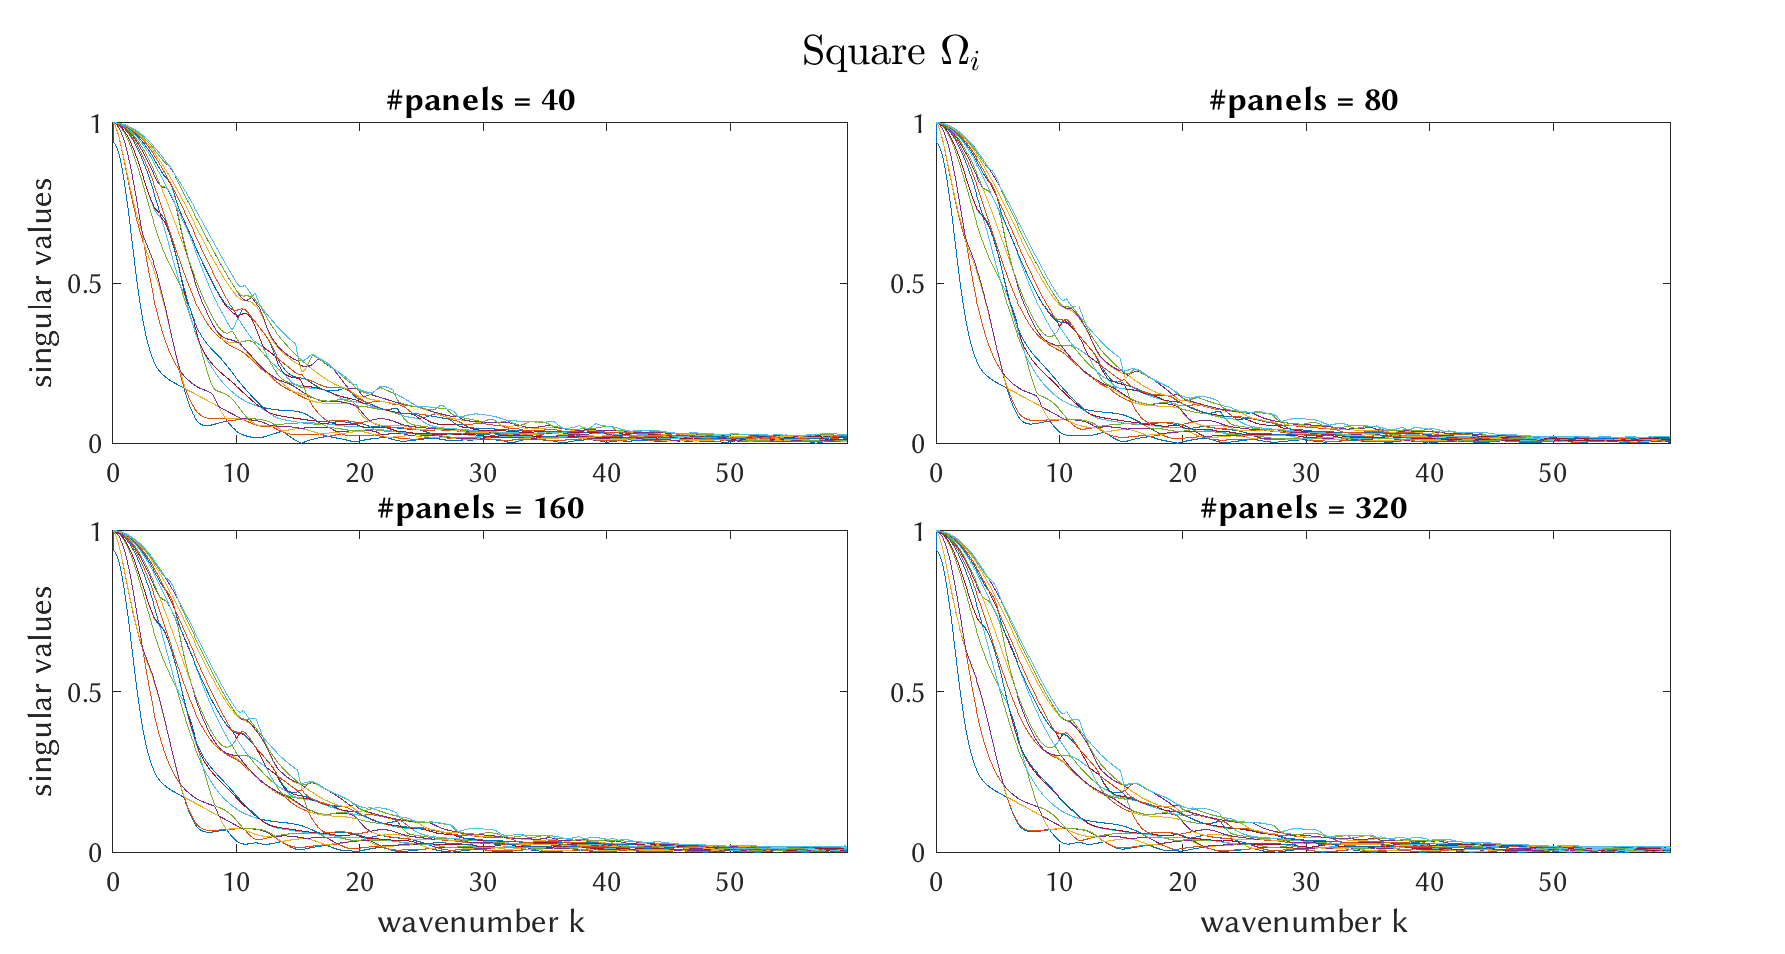
\includegraphics[width=\columnwidth]{figures/SVs_square.eps}
	\caption{ 
		Singular values computed with $\Omega_i$ being a square. 
		Convergence can be seen as was the case when $\Omega_i$ is a circle.
	}
	\label{fig:SVs_square}
\end{figure}
Although qualitatively the behaviour of the singular values is already well visible when computing with fewer panels it can also be seen that certain artefacts occur.
This can be seen well in the plot generated on the circular domain using $50$ panels.
Here there seems to be a split in the values of the two smallest singular values while when we look at the plot generated using more panels these two singular values end up having the same value.
Also it can be seen that when using only 50 panels the minima start to diverge away from the x-axis for relatively small wavenumbers $k$.

In the next sections we will look how these plots change for different refraction indices.
We will be using operators computed on 400 panels since we have seen relatively good convergence in our singular values and no breakdown in convergence in our validations of the operators.

\subsection{Varying Refraction Index}
The results are plotted for the circle in figure \ref{fig:SVs_circle_refraction} and for the square in figure \ref{fig:SVs_square_refraction}. 
The minima in the singular values seem to occur more freuqently as the refraction index $n_i$ gets farther away from one.
This applies to the singular values computed on the circle as well as on the square although on the square this seems to happen more erratically while on the circle patterns arise faster and clearer.
\begin{figure} [H]
	\centering
	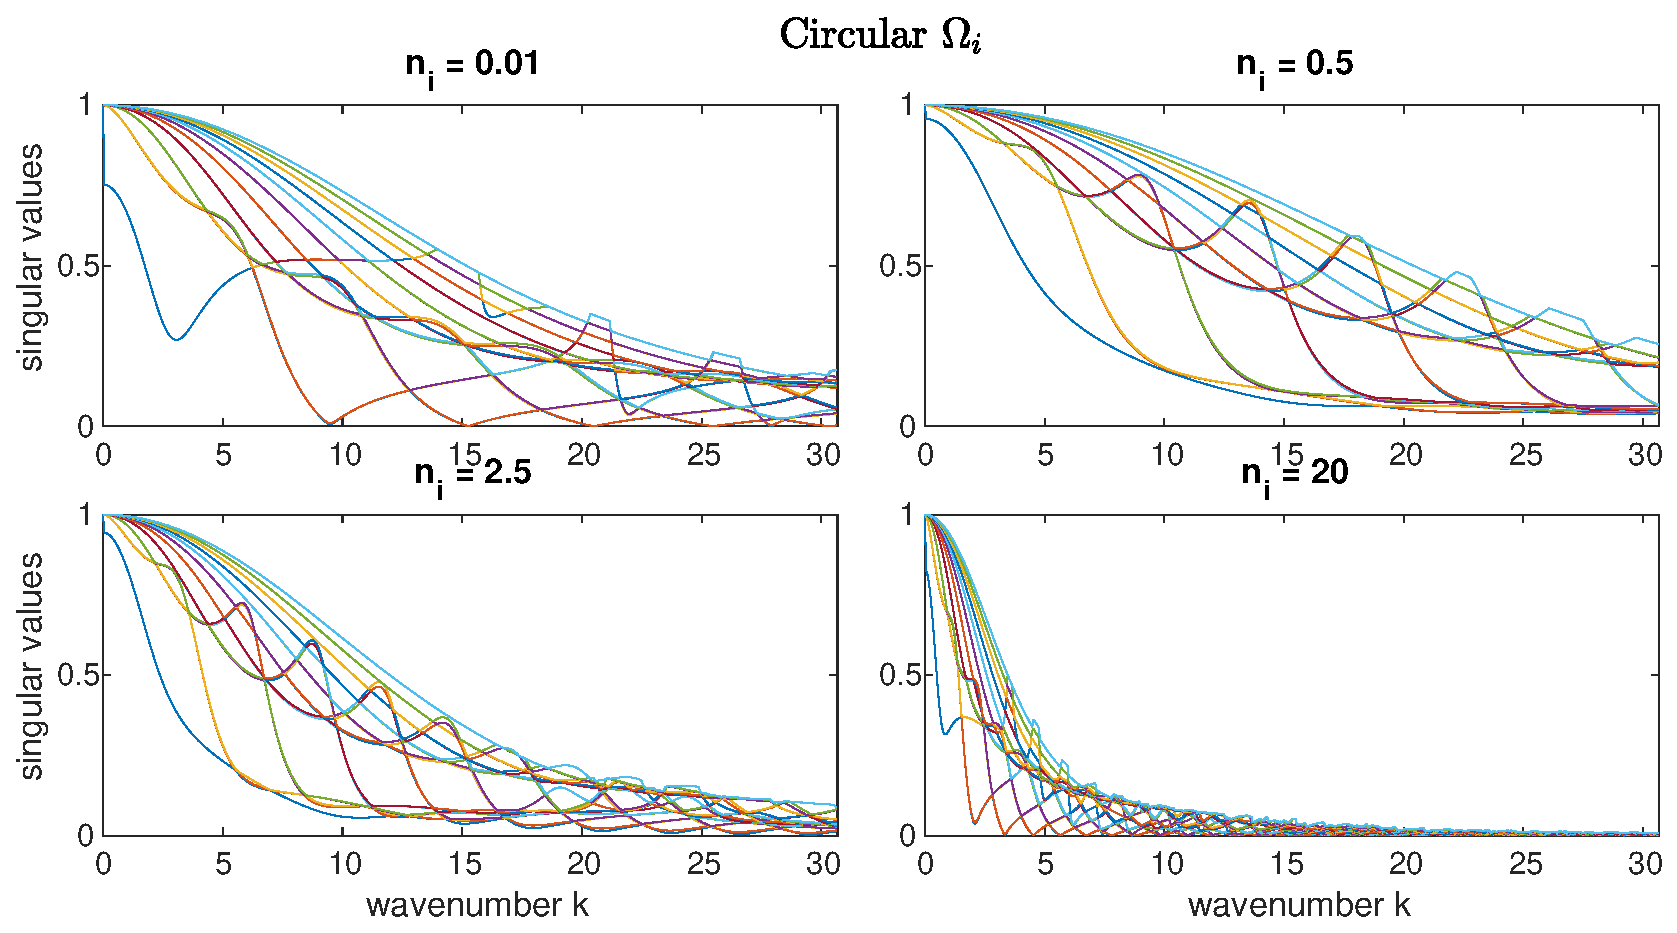
\includegraphics[width=\columnwidth]{figures/SVs_circle_refraction.eps}
	\caption{
		The 20 smallest singular values of the approximated BIOs for a circular boundary of $\Omega_i$. 
		A higher contras leads to more minima in smaller ranges of $k$.
	}
	\label{fig:SVs_circle_refraction}
\end{figure}
\begin{figure} [H]
	\centering
	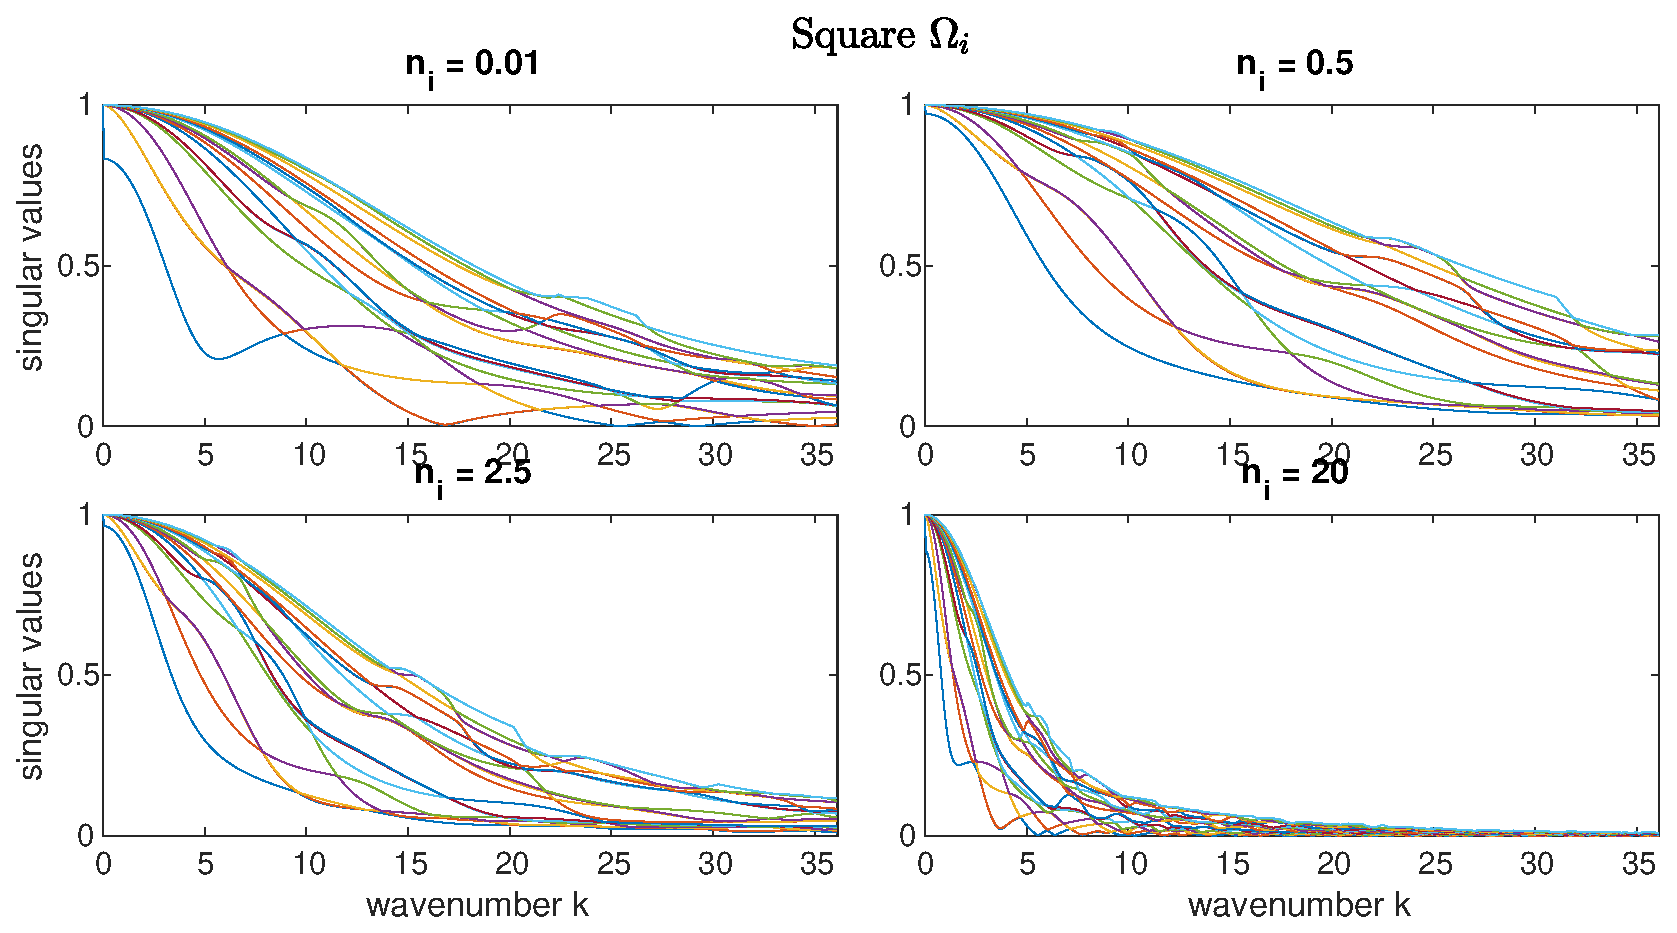
\includegraphics[width=\columnwidth]{figures/SVs_square_refraction.eps}
	\caption{ 
		The 20 smallest singular values of the approximated BIOs for a square boundary of $\Omega_i$.
		As was seen for the singular values on the circle more resonances occur in the same frequency interval as the refraction increases.
	}
	\label{fig:SVs_square_refraction}
\end{figure}
\newpage
\section{Validating Derivatives of Singular Values}
Using the algorithms from section \ref{sec:svder} we computed the first and second derivative of the smallest of the singular values that we saw in the previous sections.
To validate these derivatives we recomputed them using extrapolation and compared the results.
We will look at plots for different refraction indices here as well.
We are still computing on our baseline problem.
However we are only computing BIOs that are approximated on fifty panels.
This is because it is very costly to compute the singular values, their first and second derivative, and the derivatives by extrapolation as well.
Since our algorithms hold for arbitrary matrices having a low grade approximation of the BIOs does not matter and we can validate the algorithms regardless.
\subsection{Varying Refraction Index}
In this section we will be looking at the results for different refraction indices $n_i$.
The figure \ref{fig:derivatives_circle_refraction} shows the validation on the circle and the figure \ref{fig:derivatives_square_refraction} shows it on the square.

\begin{figure} [H]
	\centering
	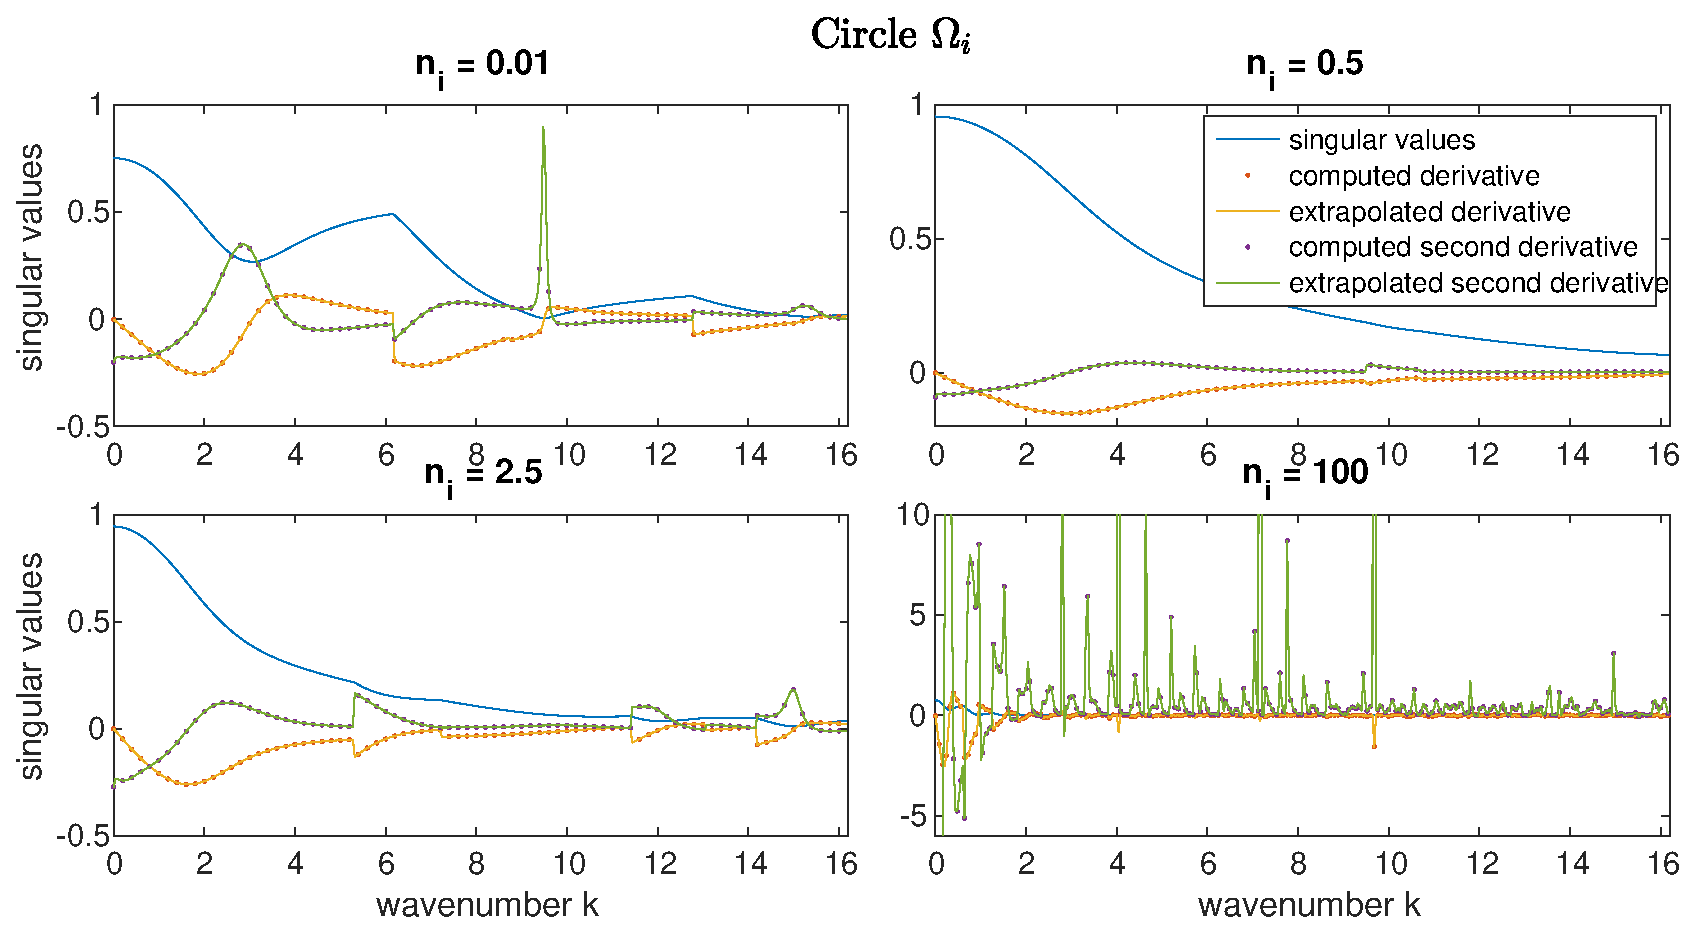
\includegraphics[width=\columnwidth]{figures/derivatives_circle_refraction.eps}
	\caption{
		This is the smallest singular value and it's derivatives computed on a circular boundary.
		In this figure and for the rest of the thesis we refer to the computed derivatives as the ones obtained by using the algorithms from section \ref{sec:svder}.
		The plots show that the computed derivatives coincide with the extrapolated derivatives almost everywhere.
	}
	\label{fig:derivatives_circle_refraction}
\end{figure}
Both figures demonstrate that our computed derivatives are accurate.
In rare cases there seem to be discrepancies at individual points to the derivatives computed by extrapolation.
We assume this is due to numerical problems in the extrapolated derivatives stemming from the fact that the smallest singular value is not a smooth function in $k$.
\begin{figure} [H]
	\centering
	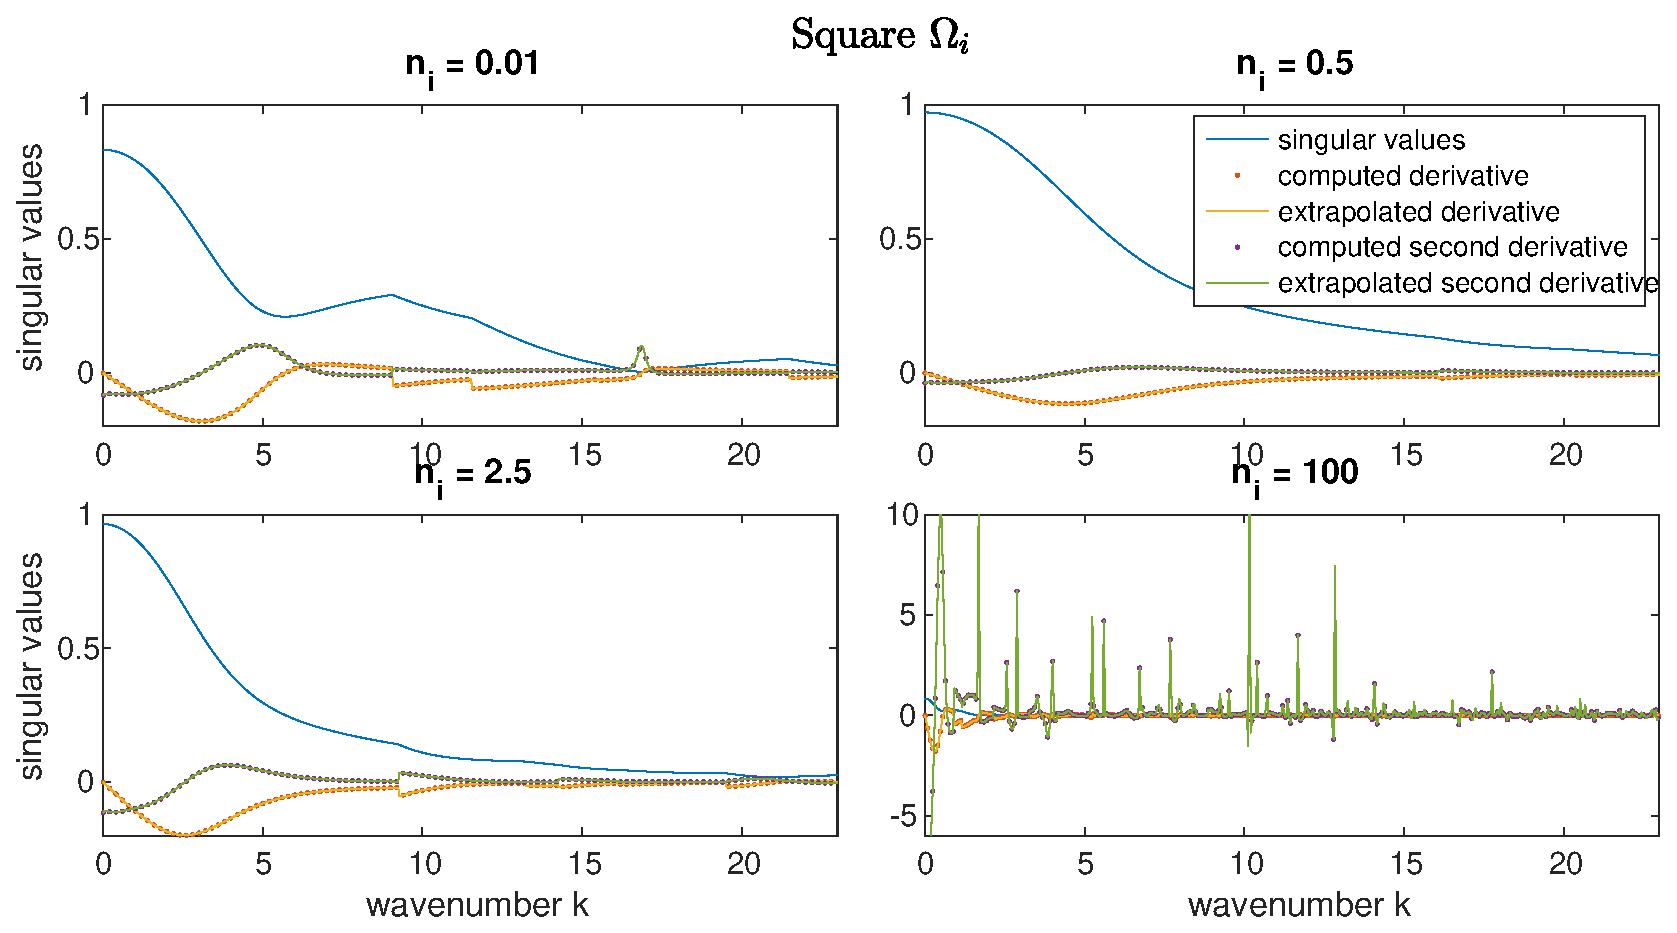
\includegraphics[width=\columnwidth]{figures/derivatives_square_refraction.eps}
	\caption{
		Here we plotted the smallest singular value and it's derivatives on the square boundary.
		As was the case for the circular boundary the computed and the extrapolated derivatives coincide almost everywhere.
	}
	\label{fig:derivatives_square_refraction}
\end{figure}

In the next section we will be using the derivatives verified here to compute the minima in the smallest singular value.

\section{Finding Minima}
Here we will be computing minima in the smallest singular value using the algorithms described in section \ref{sec:roots} applied to the singular values derivative.
Since the secant method converged towards roots completely outside of our range in many cases we will stick to the Van Wijngaarden-Dekker-Brent and the Newton-Raphson method.
To test these methods we started by taking our baseline problem on the circle and changed the refraction index to twenty.
In order to find minima we have to initialize our root finding algorithm with two values to set the interval on which to search for a root of the first derivative.
To determine how small the mesh of these intervals has to be we ran both our algorithms for different numbers of intervals.
The figure \ref{fig:roots_brent_circle_50_20} contains the results from the Van Wijngaarden-Dekker-Brent method and the figure \ref{fig:roots_newton_circle_50_20} contain the results from the Newton-Raphson method.
The results in these figures were computed with operators approximated with 50 panels.
\begin{figure} [H]
	\centering
	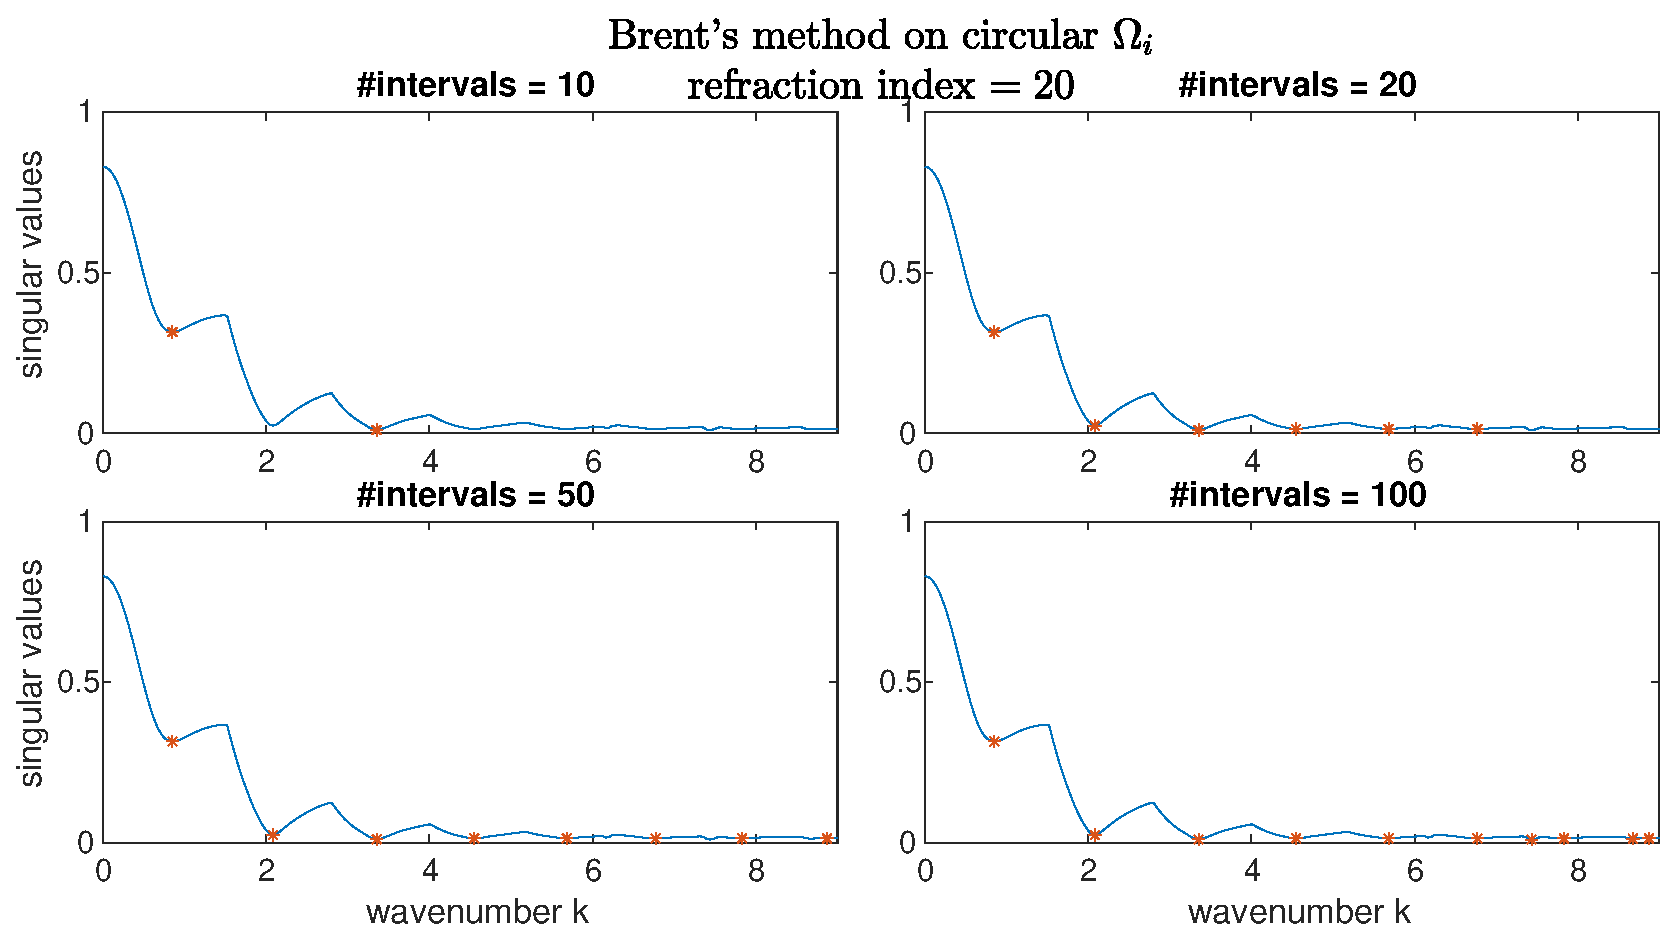
\includegraphics[width=\columnwidth]{figures/roots_brent_circle_50_20.eps}
	\caption{
		The roots found by the Van Wijngaarden-Dekker-Brent method represented as minima of the smallest singular value.
		New minima are found as the number of intervals for the root search is increased.
		One minimum remains unidentified.
	}

	\label{fig:roots_brent_circle_50_20}
\end{figure}
Both methods apparently find the same minima in the function of the smallest singular value.
As the number of intervals increase there always seem to be new minima found so a high resolution is necessary.
It can also be seen that there is a minima right after $k=6$ that never gets found.
However these small indentations seem to be artefacts stemming from the use of operators approximated on a small amount of panels.
\begin{figure} [H]
	\centering
	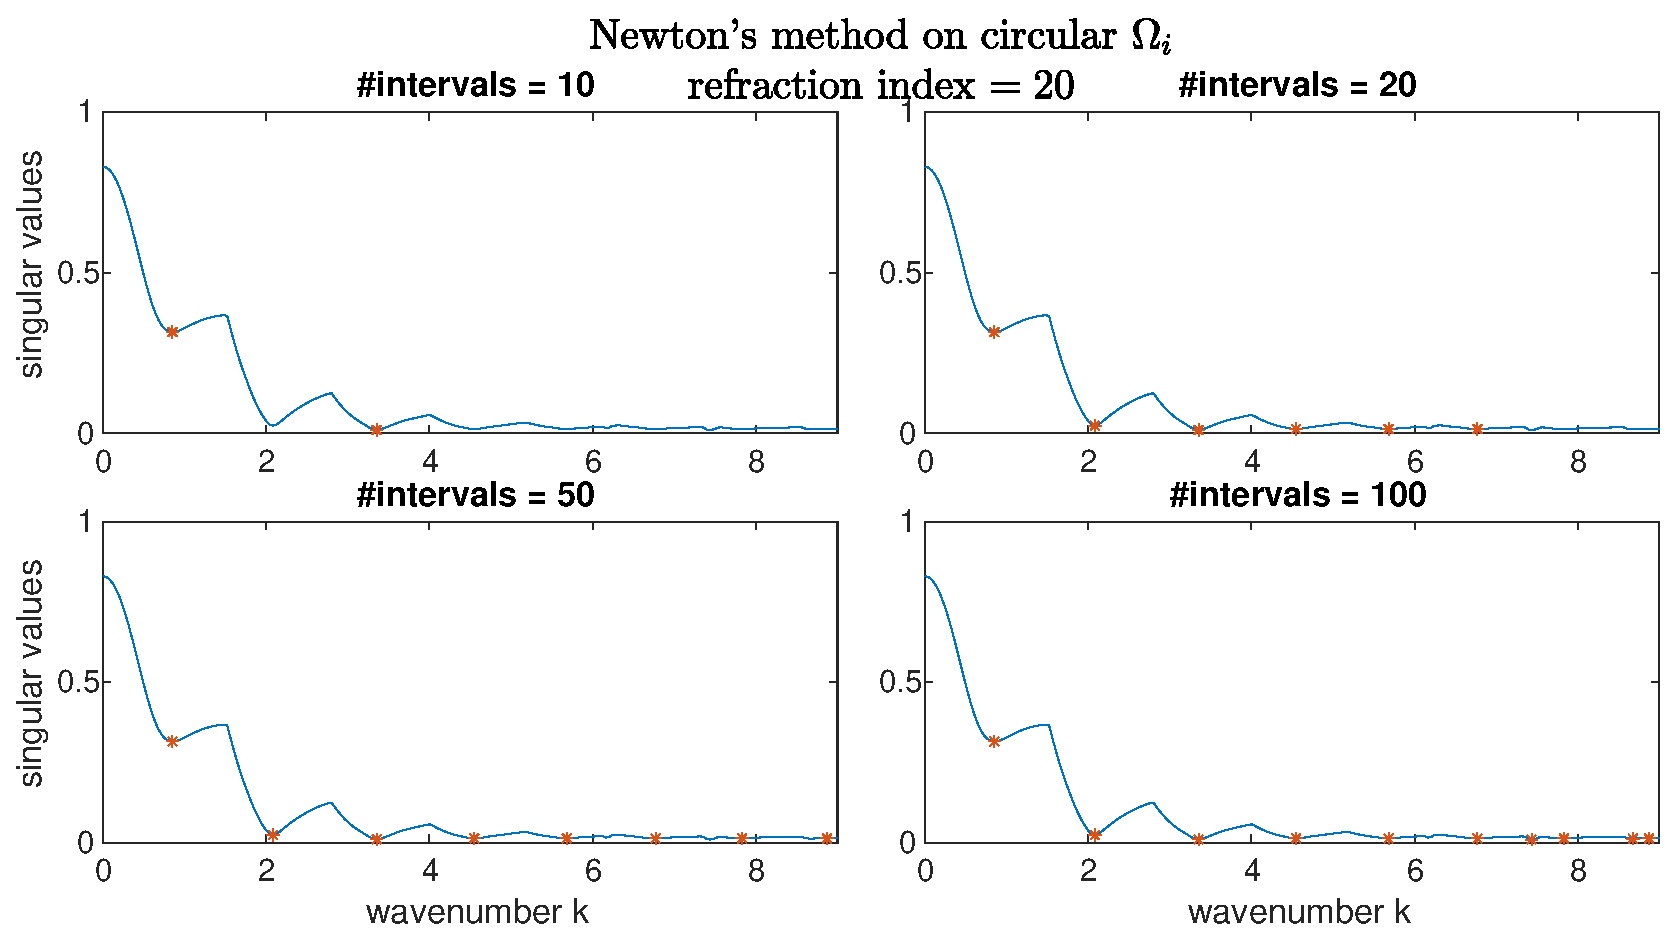
\includegraphics[width=\columnwidth]{figures/roots_newton_circle_50_20.eps}
	\caption{
		Using the Newton-Raphson method the same minima are identified as with the Van Wijngaarden-Dekker-Brent method and the same missing minimum can be seen.
	}
	\label{fig:roots_newton_circle_50_20}
\end{figure}
As can be seen in section \ref{sec:valsv} these irregularities disappear as the number of panels is increased.
Therefore it should not be a problem that these particular minima aren't always found.
To see if we get rid of the unidentified minima we recomputed the same problem with BIOs approximated on 200 panels.
The result is shown in figure \ref{fig:roots_newton_circle_200_20}.
\begin{figure} [H]
	\centering
	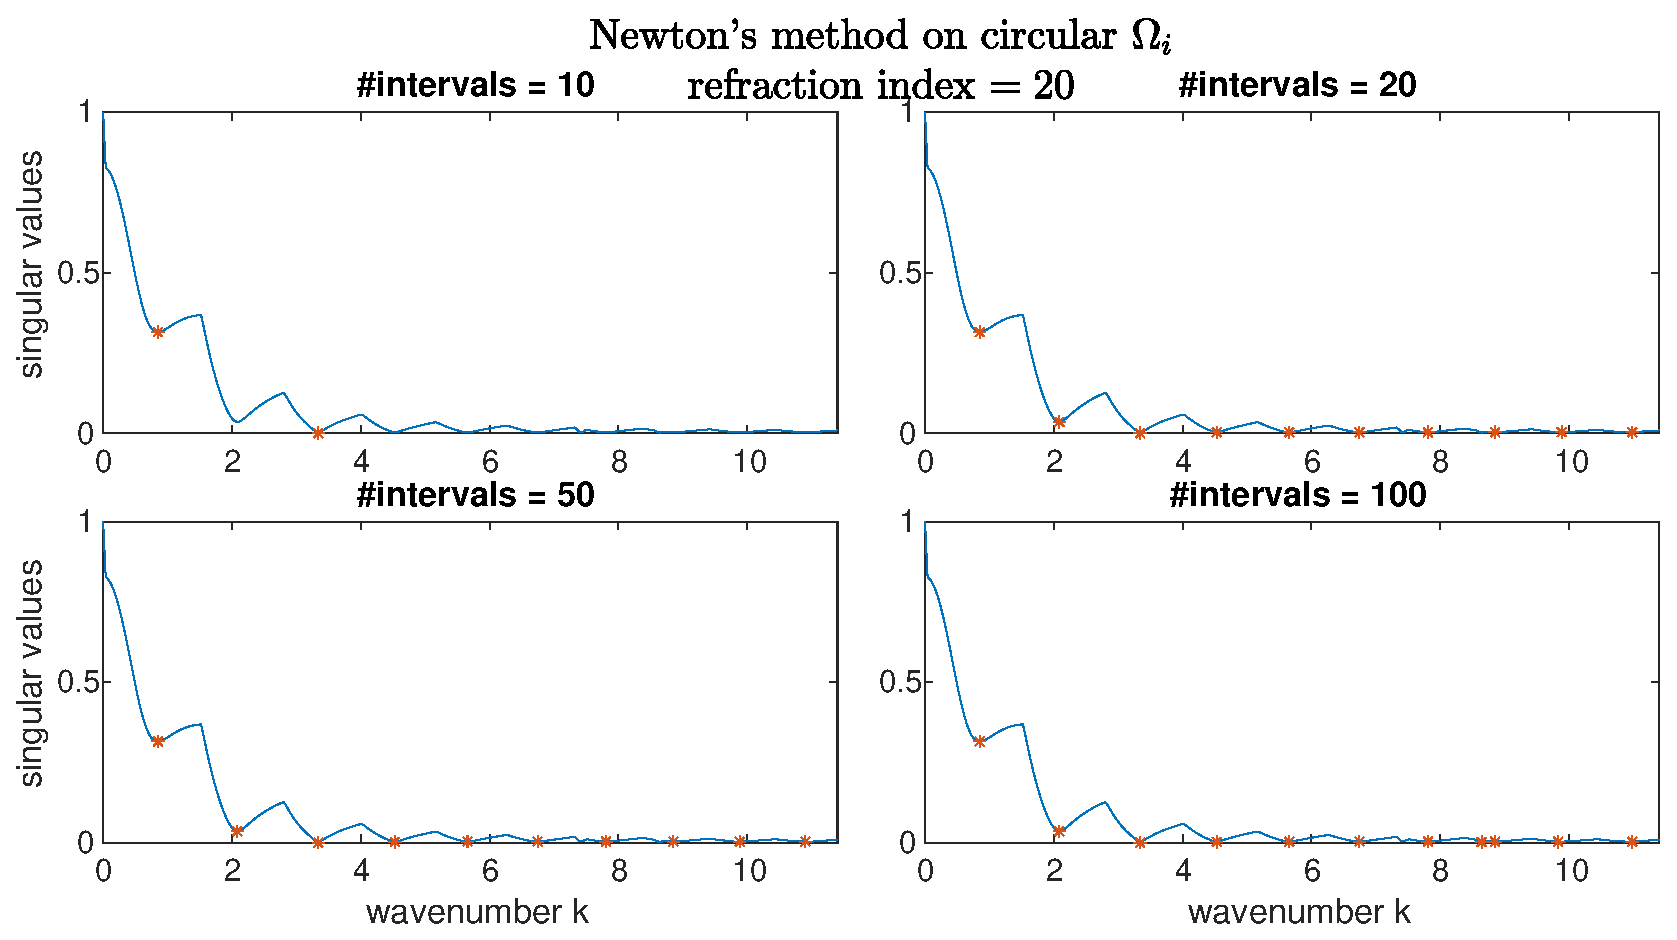
\includegraphics[width=\columnwidth]{figures/roots_newton_circle_200_20.eps}
	\caption{
		Using more panels to approximate our BIOs lets us correct errors in the smallest singular value.
		The panels necessary and the range of $k$ that can be rectified depend on the refraction index.
	}
	\label{fig:roots_newton_circle_200_20}
\end{figure}
We can see that the false minima disappears however for larger values of $k$ there still remain to be false or unidentified minima.
We can see though that increasing the number of panels for the BIOs will make the false minima disappear eventually.
For a refraction index of size $20$ however it would already take very large operators to get rid of all the errors in the smallest singular value in this range.
For a refraction index closer to one we can cover a larger range of $k$ without encountering these problems.
This can be seen in figure \ref{fig:roots_newton_circle_200_5}.
In the next section we will be comparing the efficiency of the Newton-Raphson method to the efficiency of the Van Wijngaarden-Dekker-Brent method for our specific application.

\begin{figure} [H]
	\centering
	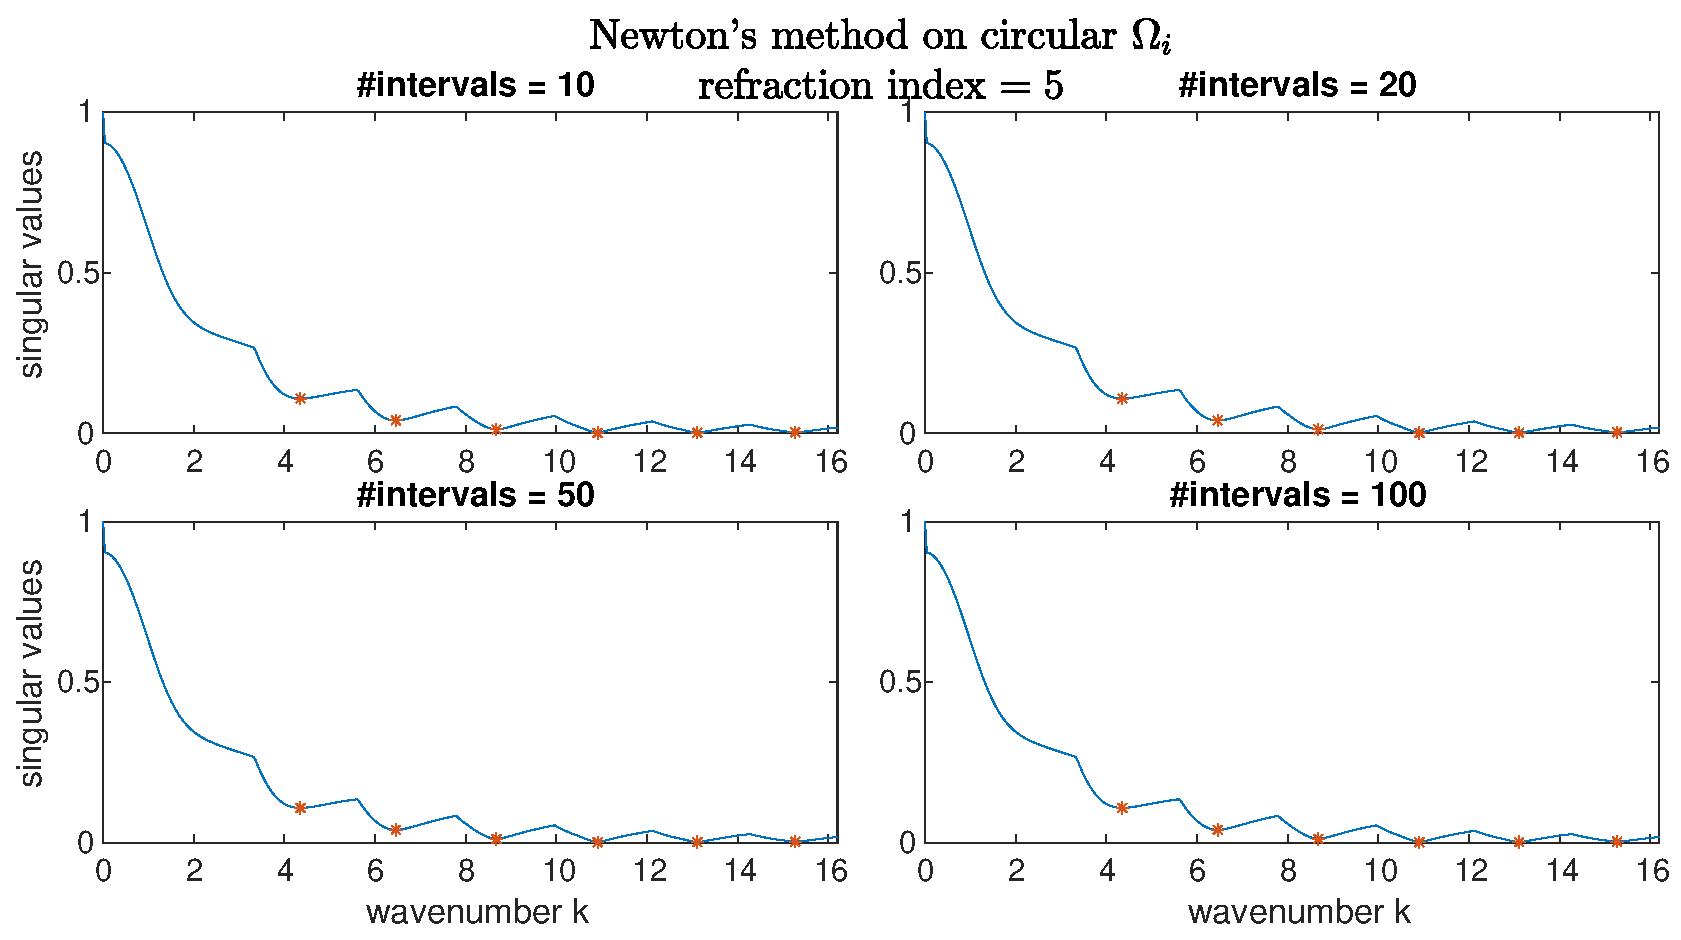
\includegraphics[width=\columnwidth]{figures/roots_newton_circle_200_5.eps}
	\caption{
		For refraction indices closer to one a larger range can be covered while remaining at 200 panels for our BIO approximation.
		The refraction index is set to five here.
	}
	\label{fig:roots_newton_circle_200_5}
\end{figure}
\section{Profiling}
As we know from section \ref{sec:roots} the convergence rate of the Newton-Raphson method is faster than that of the Van Wijngaarden-Dekker-Brent method.
We could confirm this by checking the amount of iteration the algorithms took to find the first eight minima in the baseline problem using 200 panels to approximate our operators.
The results are shown in the table \ref{tbl:conv}.
\begin{table}[H]
	\centering
	\resizebox{\columnwidth}{!}{%
		\begin{tabular}{ |c|c|c|c|c|c|c|c|c|c|c|c| } 
			\hline
			minima & \#1& \#2& \#3& \#4& \#5& \#6& \#7& \#8\\%& \#9& \#10& \#11\\ 
			\hline
			\#steps Van Wijngaarden-Dekker-Brent & 7 & 7 & 6 & 7 & 8 & 7 & 6 & 6 \\%& 5 & 6 & 6\\ 
			\#steps Newton-Raphson & 4 & 3 & 4 & 7 & 6 & 4 & 3 & 2 \\ 
			\hline
		\end{tabular}
	}
	\caption{Steps taken until convergence for first eight minima found on our baseline problem.}
	\label{tbl:conv}
\end{table}

Clearly the Newton-Raphson Method upholds the theoretical edge that it has in this regard.
However this method has to evaluate the first and the second derivative of the singular value at every iteration while the Van Wijngaarden-Dekker-Brent method only evaluates the first derivative.
Evaluating the derivatives involves computing the derivatives of the BIOs.
These are very costly operations.
The operator for which we are computing the derivatives is:
\begin{align}
	I + (A_o-A_i) \label{eq:BIOtoApprox}.
\end{align}
The dominating terms here are the approximations of the Calderón operators $A_o$ and $A_i$.
The cost of approximating the operator $I$ is negligible since it scales linearly in $\#panels$ used as opposed to quadratically.
Also for the derivatives of the operator it is dropped since it does not depend on $k$.
Each of the Calderón operators however consists of four operators as can be seen in the definition \ref{BIEtot}.
Each of those operator approximations in turn results in a matrix with $(\#panels)^2$ entries, and each of these entries has to be computed with at least $(order)^2$ evaluations of one of the kernels stated in \ref{cg}.
Some entries require even more evaluations due to the composite Gauss-Legendre quadrature rule being applied.
For the sake of simplicity we will assume a standard quadrature rule for all entries as an estimate.
This leads to the approximation of \ref{eq:BIOtoApprox} costing about:
\begin{equation}
	N := 2\cdot4\cdot(\#panels)^2\cdot(order)^2
\end{equation}
kernel evaluations.
That is approximating two Calderón operators, consisting of four operators each, resulting in matrices with $(\#panels)^2$ entries, each requiring $(order)^2$ kernel evaluations to be computed. 
The approximations of the derivatives of the operator \ref{eq:BIOtoApprox} is mostly the same apart from the kernel evaluations being slightly costlier.
Using these estimates it is safe to say that the evaluation of the singular value derivatives is the dominating part of an iteration in both our root finding algorithms.
In fact measuring the time spent in the computation of the singular values versus the time spent overall finding a root for the computations listed in \ref{tbl:conv}, we saw that over $99\%$ of the time was spent computing the BIOs and extracting the singular values.
Checking the algorithms from \ref{sec:roots} tells us that computing the derivative of singular values requires to compute the matrix of interest and it's first derivative.
Computing the second derivative requires the matrix and it's first two derivatives.
This means a Newton-Raphson iteration, which needs to compute the second derivative of the singular value, costs about $1.5$ times as much as a Van Wijngaarden-Dekker-Brent Iteration that only computes the first derivative.
This is assuming that the operator \ref{eq:BIOtoApprox} and it's derivatives all cost about $N$ equivalent kernel evaluations to compute, and that the cost of the extracting of the derivatives from the computed BIOs is negligible.

In table \ref{tbl:time} we listed the overall time taken to find the roots by the different algorithms in seconds for the same roots as listed in \ref{tbl:conv}.

\begin{table}[H]
	\centering
	\resizebox{\columnwidth}{!}{%
		\begin{tabular}{ |c|c|c|c|c|c|c|c|c|c|c|c| } 
			\hline
			minima & \#1& \#2& \#3& \#4& \#5& \#6& \#7& \#8\\%& \#9& \#10& \#11\\ 
			\hline
			\#(s) Van Wijngaarden-Dekker-Brent & 3332 & 3721 & 3277 & 3483 & 3953 & 3710 & 3138 & 2798 \\%& 5 & 6 & 6\\ 
			\#(s) Newton-Raphson & 4525 & 3808 & 5049 & 7667 & 6138 & 4204 & 3473 & 2402 \\ 
			\hline
		\end{tabular}
	}
	\caption{Time spent in seconds until convergence for first eight minima found on our baseline problem.}
	\label{tbl:time}
\end{table}
We can see that the Van Wijngaarden-Dekker-Brent method fairs quite a bit better than the Newton-Raphson method in most cases, even in cases where it needs more than $1.5$ times as many iterations to converge.
This is due to the fact that the extracting of the derivatives from the computed operators is actually not negligible contrary to what we assumed earlier.
For both algorithms presented in section \ref{sec:svder} an eigenvalue decomposition of the Wielandt matrix is required.
However for the second derivative algorithm matrix inverses have to be computed as for the first derivative algorithm only matrix-vector and vector-vector products are computed.
Furthermore the operator \ref{eq:BIOtoApprox}, it's first derivative, and it's second derivative all have slightly different kernels that need to be evaluated $N$ times with kernels getting more expensive to compute with each derivative.
So even when the Newton-Raphson method converges faster than the Van Wijngaarden-Dekker-Brent method, in a magnitude that would allow the $1.5$ times higher time spent computing operators to be tolerable, it still is not faster due to the high cost, scaling as $(\#panels)^3$, of the matrix inversions it has to compute and the higher cost of the kernels that have to be evaluated.
Therefore the Van Wijngaarden-Dekker-Brent method is actually more effective in our case despite it's lower convergence rate.

In the following last chapter we will give a conclusion to this thesis.

\chapter{Conclusion}
To conclude our work here we will summarize the lessons learned from chapter \ref{chap:numres}.
First off we saw that we could get the best convergence rate for our baseline case when we set $order=11$ for our quadrature rules.
It could be argued that in some cases, when a known acceptable error is available, a lower order could be set for efficiency.
However we can't give any exact advice on that at this point.
Furthermore we could determine that our algorithms were mostly stable except for certain edge cases when varying the wavenumber, the refraction index, or the incoming wave and the resulting wave thereof.

After testing the optimal order for our quadrature rules we went on to investigate the computed singular values of our approximated BIOs.
Here we saw that the qualitative behaviour of the smallest singular values was already visible for operators computed with very few panels.
It could also be seen though that certain artefacts did occur for operators computed with a low panel count especially for larger wavenumbers.
For refraction indices strongly differing from 1 the patterns in the singular values became more erratic suggesting that here computing with more rather than less panels would be favourable as well.

We could validate that the algorithms for computing the derivatives of singular values described in section \ref{sec:svder} don't add any meaningful numerical errors.
Here the number of panels used is completely irrelevant.
For root finding however we could see that the artefacts seen in singular values of operators approximated with few panels could become troublesome.
The problems we encountered specifically related to refraction indices far away from one and increasing values of $k$.
Increasing the number of panels for our BIO approximations we could get rid of some of the problems we ran into.
However outside a certain range around one for the refraction index and larger values of $k$ it becomes unfeasible to run these computations over meaningful ranges since the approximated operators would need to be computed with an immense number of panels.
Within reasonable ranges of $k$ and for refraction indices not too far from one, minima in the smallest singular value could be located accurately.

Finally we saw that the Van Wijngaarden-Dekker-Brent method actually compared favourably to the Newton-Raphson method despite it's lower convergence rate.
This is due to that the Van Wijngaarden-Dekker-Brent method only relies on the first derivative of the singular value which can we can compute more efficiently than the second derivative.

As a general rule of thumb we advise to compute resonances of the Helmholtz transmission problem using 11 as the order of the Gauss-Legendre quadrature rules.
As for how to set the amount of panels used to approximate the BIOs, this is dependent on the range of $k$ and the refraction index.
To get reliable results it would be good to start out with a small number of panels and increase it until either stability with respect to the found minima in the smallest singular value has been reached or until the available compute power is depleted.
The method of choice for determining the minima through root finding for the derivative should be the Van Wijngaarden-Dekker-Brent method. 

Future work pertaining to this thesis would be to apply the developed algorithms to real world problems and see how well scatterer resonances can be identified using our code.
Furthermore attempts were made to improve the performance of identifying minima by using a more adaptive algorithm, based on parabolic approximation, that is not bound to rigid evaluations along a mesh.
At this moment the algorithm is not stable but with some modification and the correct parametrization the performance improvement might still be achieved.

% This displays the bibliography for all cited external documents. All references have to be defined in the file references.bib and can then be cited from within this document.
\bibliographystyle{IEEEtran}
\bibliography{references/references}

% This creates an appendix chapter, comment if not needed.
\appendix
\chapter{Usage} \label{chap:usage}
The library is located at:

\url{https://github.com/DiegoRenner/HelmholtzTransmissionProblemBEM}.

It can be configured by running \verb|cmake CMakeLists.txt| in the base directory
or \verb|cmake ..| in a subdirectory for an out-of-source build.
This should automatically install the Eigen library \cite{eigenweb} for matrix computations if it is not already available.
The same goes for the complex\_bessel library \cite{cb} that is used for passing complex arguments to the Hankel and Bessel functions.
To generate the documentation \LaTeX and \verb|doxygen| have to be installed.
Running CMake also configures \verb|make| targets.
These can then be built by running 

\verb|make <target_name>|.

The compiled binary can be found in the \verb|bin| directory.
We will show how the built targets are to be used.

\cprotect\section{\verb|doxygen_HelmholtzTransmissionProblemBEM|}
This target generates a documentation of the library in the \verb|doxygen/generated_doc| directory.
The documentation can be browsed using any common browser.

\cprotect\section{\verb|dirichlet_example|}
This target builds a script that computes the solution to a Dirichlet problem
using first kind direct BIEs.
No command line parameters are necessary.
Once built the script can be run as follows: 
\begin{verbatim}
/path/to/library/bin/dirichlet_example.
\end{verbatim}
The user will be updated over the residual error in the euclidean norm of the computed FEM-space interpolation coefficients to the known FEM-space interpolation coefficients for the current number of panels through the command line.

\cprotect\section{\verb|neumann_example|}
This target builds a script that computes the solution to a Neumann problem
using first kind direct BIEs.
No command line parameters are necessary.
Once built the script can be run as follows: 
\begin{verbatim}
/path/to/library/bin/neumann_example.
\end{verbatim}
The user will be updated over the residual error in the euclidean norm of the computed FEM-space interpolation coefficients to the known FEM-space interpolation coefficients for the current number of panels through the command line.

\cprotect\section{\verb|parabolic_approximation|}
This target builds a script that tries to find minima in the smallest singular values
of the Galerkin BEM approximated solutions operator for the second-kind direct BIEs of 
the Helmholtz Transmission problem.
The minima are searched for using a parabolic approximation
based on evaluating the smallest singular values and their first
two derivatives.
The results are written to disk.
No command line arguments are necessary.
The script can be run as follows:
\begin{verbatim}
/path/to/library/bin/parabolic_approximation <outfile>.
\end{verbatim}
In the file the first column contains the initial point used for the parabolic approximation.
The next three columns contain the function value and the first two derivatives at the initial point that were used to compute the parabolic approximation.
The user also will get updates on the current best approximation for a minima and the value of the first derivatie at this point through the command line if \verb|-DCMDL| is set.

\cprotect\section{\verb|roots_brent_circle|}
This target builds a script that computes minima in the smallest singular value of the
Galerkin BEM approximated solutions operator for the second-kind direct BIEs of the Helmholtz
transmission problem using the Van Wijngaarden-Dekker-Brent method.
The scatterer is set to be a circle.
The results are written to disk.
The script can be run as follows:
\begin{verbatim}
/path/to/library/bin/roots_brent_circle <radius of circle> 
	<refraction inside> <refraction outside> 
	<initial wavenumber> <#grid points for root search> 
	<#panels> <order of quadrature rule> <outputfile>.
\end{verbatim}
The resulting file will contain the left boundary of the interval used to compute the root in the first column. 
Then in the next three columns will be the point, the function value and the derivative at which the root was found.
The last column will contain the number of iterations used to find the root.
If no root was found the last four columns will be set to \verb|NAN|.
The user will be updated through the command line about the progress of the algorithm if \verb|-DCMDL| is set.

\cprotect\section{\verb|roots_brent_square|}
This target builds a script that computes minima in the smallest singular value of the
Galerkin BEM approximated solutions operator for the second-kind direct BIEs of the Helmholtz
transmission problem using the Van Wijngaarden-Dekker-Brent method.
The scatterer is set to be a square.
The results are written to disk.
The script can be run as follows:
\begin{verbatim}
/path/to/library/bin/roots_brent_circle <half side length of square> 
	<refraction inside> <refraction outside> 
	<initial wavenumber> <#grid points for root search> 
	<#panels> <order of quadrature rule> <outputfile>.
\end{verbatim}
The resulting file will contain the left boundary of the interval used to compute the root in the first column. 
Then in the next three columns will be the point, the function value and the derivative at which the root was found.
The last column will contain the number of iterations used to find the root.
If no root was found the last four columns will be set to \verb|NAN|.
The user will be updated through the command line about the progress of the algorithm if \verb|-DCMDL| is set.

\cprotect\section{\verb|roots_newton_circle|}
This target builds a script that computes minima in the smallest singular value of the
Galerkin BEM approximated solutions operator for the second-kind direct BIEs of the Helmholtz
transmission problem using the Newton-Raphson method.
The scatterer is set to be a circle.
The results are written to disk.
The script can be run as follows:
\begin{verbatim}
/path/to/library/bin/roots_newton_circle <radius of circle> 
	<refraction inside> <refraction outside> <initial wavenumber> 
	<#grid points for root search> <#panels> 
	<order of quadrature rule> <outputfile>.
\end{verbatim}
The resulting file will contain the left boundary of the interval used to compute the root in the first column. 
Then in the next three columns will be the point, the function value and the derivative at which the root was found.
The last column will contain the number of iterations used to find the root.
If no root was found the last four columns will be set to \verb|NAN|.
The user will be updated through the command line about the progress of the algorithm if \verb|-DCMDL| is set.

\cprotect\section{\verb|roots_newton_square|}
This target builds a script that computes minima in the smallest singular value of the
Galerkin BEM approximated solutions operator for the second-kind direct BIEs of the Helmholtz
transmission problem using the Newton-Raphson method.
The scatterer is set to be a square.
The results are written to disk.
The script can be run as follows:
\begin{verbatim}
/path/to/library/bin/roots_newton_circle <half side length of square> 
	<refraction inside> <refraction outside> <initial wavenumber> 
	<#grid points for root search> <#panels> 
	<order of quadrature rule> <outputfile>.
\end{verbatim}
The resulting file will contain the left boundary of the interval used to compute the root in the first column. 
Then in the next three columns will be the point, the function value and the derivative at which the root was found.
The last column will contain the number of iterations used to find the root.
If no root was found the last four columns will be set to \verb|NAN|.
The user will be updated through the command line about the progress of the algorithm if \verb|-DCMDL| is set.

\cprotect\section{\verb|sv_circle|}
This target builds a script that computes the singular values
of the Galerkin BEM approximated BIO for the
second-kind direct BIEs of the Helmholtz
transmission problem.
The scatterer is set to be a circle.
The results are written to file.
The script can be run as follows:
\begin{verbatim}
/path/to/library/bin/sv_circle <radius of circle> 
	<refraction inside> <refraction outside> <initial wavenumber>
	<#panels> <order of quadrature rule> <outputfile>
\end{verbatim}
The resulting file will contain the value of $k$ in the first column.
The rest of the columns contain the singular values from smallest to largest for this $k$.
The user will be updated through the command line about the progress of the algorithm if \verb|-DCMDL| is set.

\cprotect\section{\verb|sv_square|}
This target builds a script that computes the singular values
of the Galerkin BEM approximated BIO for the
second-kind direct BIEs of the Helmholtz
transmission problem.
The scatterer is set to be a square.
The results are written to file.
The script can be run as follows:
\begin{verbatim}
/path/to/library/bin/sv_circle <half of side length of square> 
	<refraction inside> <refraction outside> <initial wavenumber>
	<#panels> <order of quadrature rule> <outputfile>
\end{verbatim}
The resulting file will contain the value of $k$ in the first column.
The rest of the columns contain the singular values from smallest to largest for this $k$.
The user will be updated through the command line about the progress of the algorithm if \verb|-DCMDL| is set.


\cprotect\section{\verb|sv_derivative_verification_circle|}
This target builds a script that verifies the derivatives of the singular
values of the Galerkin BEM approximated BIO for the
second-kind direct BIEs of the Helmholtz transmission problem
using extrapolation.
The scatterer is set to be a circle.
The results are written to file.
The script can be run as follows:
\begin{verbatim}
/path/to/library/bin/sv_derivative_verification_circle 
	<radius of circle> <refraction inside> <refraction outside> 
	<initial wavenumber> <#panels> <order of quadrature rule> <outputfile>
\end{verbatim}
The resulting file will contain the value of $k$ in the first column.
The second column will contain the value of the smallest singular value at this $k$.
Then the columns will contain the computed derivative, the extrapolated derivative, the computed second derivative and the extrapolated second derivative in this order.
The user will be updated through the command line about the progress of the algorithm if \verb|-DCMDL| is set.

\cprotect\section{\verb|sv_derivative_verification_square|}
This target builds a script that verifies the derivatives of the singular
values and their derivatives of the Galerkin BEM BIO for the
second-kind direct BIEs of the Helmholtz transmission problem
using extrapolation.
The scatterer is set to be a square.
The results are written to file.
The script can be run as follows:
\begin{verbatim}
/path/to/library/bin/sv_derivative_verification_circle 
	<half side length of square> <refraction inside> 
	<refraction outside> <initial wavenumber> <#panels> 
	<order of quadrature rule> <outputfile>
\end{verbatim}
The resulting file will contain the value of $k$ in the first column.
The second column will contain the value of the smallest singular value at this $k$.
Then the columns will contain the computed derivative, the extrapolated derivative, the computed second derivative and the extrapolated second derivative in this order.
The user will be updated through the command line about the progress of the algorithm if \verb|-DCMDL| is set.

\cprotect\section{\verb|sv_derivative_full|}
This target builds a script that computes the singular values and
their first two derivatives of the Galerkin BEM
approximated BIO for the second-kind direct BIEs of the Helmholtz
transmission problem.
Minima in the smallest singular value are determined as well
by use of the Newton-Raphson method.
The scatterer is set to be a circle.
The results are written to file.
The script can be run as follows:
\begin{verbatim}
/path/to/library/bin/sv_derivative_full <radius of circle> 
	<refraction inside> <refraction outside> <initial wavenumber>
	<#panels> <order of quadrature rule> <outputfile>
\end{verbatim}
The resulting file will contain the value of $k$ in the first column.
Then the singular values and their first two derivatives at $k$ will be listed from smallest to largest in the columns.
The singular values and their derivatives occupy three neighbouring columns.
The final three columns will contain the value of the root, the value of the first derivative at the root and the number of iterations taken to find the root in the interval between the current and the next evaluation point.
If no root was found these three columns will contain \verb|NAN|.
The user will be updated through the command line about the progress of the algorithm if \verb|-DCMDL| is set.

\cprotect\section{\verb|transmission_problem_verification|}
This target builds a script that computes solutions to
the analytically solvable case of the Helmholtz transmission
problem where the scatterer is a circle using second-kind direct
BIEs and Galerkin BEM.
The results are written to file.
The script can be run as follows:
\begin{verbatim}
/path/to/library/bin/transmission_problem_verification 
	<radius of circle> <#coeffs for series expansion of solution> 
	<refraction inside> <refraction outside> <initial wavenumber>
	<order of quadrature rule> <outputfile>
\end{verbatim}
This output file will contain two columns.
The first will contain the current panel size.
The second will contain the residual error in the euclidean norm of the computed FEM-space interpolation coefficients to the known FEM-space interpolation coefficients for the current number of panels.
The user will be updated through the command line about the progress of the algorithm if \verb|-DCMDL| is set.

\chapter{Root Finding Algorithms}
\section{Van Wijngaarden-Dekker-Brent Method}
\lstinputlisting[language=C++, caption={This algorithm from \cite{rf} implements the Van Wijngaarden-Dekker-Brent method. It can be seen that each iteration contains exactly one function evaluation at line \texttt{88}.}, label={code:zbrent}]{code/zbrent.cpp}
\section{Newton-Raphson Method}
\lstinputlisting[language=C++, caption={This algorithm implements from \cite{rf} implements the Newton-Raphson method. The single function and derivative evaluation per iteration can be seen in line \texttt{81} through \texttt{83}.}, label={code:rtsafe}]{code/rtsafe.cpp}

\chapter{Introducing a Competitive Eigensolver}
In the first implementation of the HelmholtzTransmissionProblemBEM library the solver used to compute the eigenvalues of the solutions operators Wielandt matrix was the Eigen library's eigensolver.
This is a direct eigensolver relying on the Schurdecomposition which in turn has complexity $\mathcal{O}(n^3)$, where $n$ is the size of the Wielandt matrix.
To lower the order of complexity a second approach was tried using the Arnoldi algorithm. 
In contrast to the direct solver implemented by Eigen, the Arnoldi algorithm is an iterative method.
It usually converges within in a few steps leaving it's complexity to be dominated by the complexity $\mathcal{O}(n^2)$ of the LU-decomposition and the Hessenberg-QR-decomposition.
These are used in each iteration or at the end of each run respectively.

\section{The Arnoldi Algorithm}
The Arnoldi Algorithm gives us a similarity transformation $\mathbf{A}=\mathbf{QHQ}^H$ of the matrix $\mathbf{A}$, where $\mathbf{H}$ is an upper Hessenberg matrix and $\mathbf{Q}$ is unitary.
This transformation is generated iteratively while creating a Krylov space $\mathcal{K}^{m}(\mathbf{q}_0, \mathbf{A})$ using the following iteration rule:
\begin{align}
	&\mathbf{q_{k+1}}&  &\leftarrow& &\mathbf{A}\mathbf{q}_{k}& & \label{eq:arit1}\\
	&\mathbf{q_{k+1}}&  &\leftarrow& &\mathbf{q}_{k+1} - \sum_{i=1}^{k} (\mathbf{q}_i^H \cdot \mathbf{q}_{k+1}) \mathbf{q}_i& & \text{(orthogonalize)}\\
	& \text{if } ||\mathbf{q}_{k+1}||=0 \text{: stop} \span\span\span\span& &\text{(stopping criteria)} \\
	& \mathbf{q}_{k+1}& &\leftarrow& &\frac{\mathbf{q}_{k+1}}{||\mathbf{q}_{k+1}||}& &\text{(normalize)} \label{eq:arit2}
\end{align}
for $k=0,1,...,m$. $\mathbf{q}_0$ is a random vector of length $1$ and all resulting vectors form an orthonormal basis of $\mathcal{K}^m(\mathbf{q}_0,\mathbf{A})$.
The matrix $\mathbf{Q}$'s columns are set to be the vectors $\mathbf{q}_k$ and the entries of the Hessenberg matrix $\mathbf{H}$ are given by:
\begin{align}
	\mathbf{H_{i,j}}& = \mathbf{q}_i^H \cdot \mathbf{q}_{j+1},& i \leq j+1 \\
	\mathbf{H_{i,j}}& = 0,& i \leq j+1.
\end{align}

The stopping criteria is set since at this point the generated Krylov space is invariant under $A$, meaning no new direction will be added with further iterations.
Running the algorithm to completion means the Eigenvalues of $\mathbf{A}$ and $\mathbf{H}$ are identical. 

In practice the stopping criteria is usually only fulfilled for a $k$ close to $n$.
This means we would get a complexity of $\mathcal{O}(n^3)$ since we would have to do around $n$ iterations, each with a $matrix\times vector$ product of complexity $\mathcal{O}(n^2)$.
The Arnoldi iteration (equations \ref{eq:arit1}-\ref{eq:arit2}) gives us the relationship:

\begin{equation}
	\mathbf{AQ}_k = \mathbf{Q}_k\mathbf{H}_k + \mathbf{h}_{k+1,k}\mathbf{q}_{k+1}\mathbf{e}_k^H
\end{equation}

where $\mathbf{Q}_k$ and $\mathbf{H}_k$ are the matrices generated after $k$ iterations.
This relationship allows us to approximate how close we are to finding the eigenvalues and eigenvectors of $\mathbf{A}$ at each iteration.
In order to describe this approximation let us define $\mathbf{y}_i^{(k)}$ and $\lambda_i^{(k)}$ as an eigenvector and the corresponding eigenvalue of $\mathbf{H}_k$. 
For the so called Ritz pair $(\mathbf{u}_i^{(k)},\lambda_i^{(k)})=(\mathbf{V}_k\mathbf{y}_i^{(k)},\lambda_i^{(k)})$ then the following holds:

\begin{equation}
	||(\mathbf{A}-\lambda_i^{(k)}\mathbf{I})\mathbf{u}_i^{k}||_2 = \mathbf{h}_{k+1,k} |\mathbf{e}_k^H\mathbf{y}_i^{(m)}|.	
\end{equation}

This allows us to replace the strict stopping criteria by one conditioned on $\mathbf{h}_{k+1,k} |\mathbf{e}_k^H\mathbf{y}_i^{(m)}|$ being small.
In practice this often leads to the algorithm terminating for $m \ll n$ which in turn gives a complexity of $\mathcal{O}(n^2)$. \cite{doi:10.1137/1.9781611970739.ch6} 
From here on out we will refer to the quantity $\mathbf{h}_{k+1,k} |\mathbf{e}_k^H\mathbf{y}_i^{(m)}|$ as the accuracy (with which the Arnoldi algorithm is executed).


\section{Implicitly Restarted Arnoldi}
We are using the arpackpp\cite{arpackpp} library's implementation of the Arnoldi algorithm.
This is an IRA (Implicitly Restarted Arnoldi) implementation.
Restarted Arnoldi implementations discard some of the generated Krylov space every couple of steps.
This saves on computational and memory resources since fewer vectors have to be considered when reorthogonalizing and therefore also fewer vectors have to be stored.

In order not to lose any useful information however it is important to choose which part of the space to discard and which one to keep carefully.
Applying a shifted QR-decomposition to the Hessenberg matrix $\mathbf{H}$ gives a transformation matrix than can be used to suppress unwanted directions in the Krylov space while keeping the ones we are interested in.
Unwanted directions being the ones that don't contribute to the span of the Eigenvectors we are looking for.
In order to know what this span could be it's approximated with the previously generated Krylov space.

\section{Using arpackpp and Validating the Results}\label{sec:first_results}
Arpackpp is a C++ wrapper that allows access to the Fortran arpack\cite{arpackweb} Arnoldi implementations through C++.
It uses a reverse communications interface allowing the user to apply the IRA only by providing the appropriate $(matrix\times vector)$ product.
In our case this product would be of the form:
\begin{align}
	\mathbf{W}^{-1} \mathbf{q}_k = \mathbf{q}_{k+1}.
\end{align}
where $W$ is the Wielandt matrix of our solutions operator.
To avoid the explicit inverse a LU-decomposition was used.

In order to validate our results from arpackpp we compared a series of computed singular values for a Helmholtz Transmission Problem.
The Scattering Transmission Problem was computed with the inner and outer refraction indices being $c_i=20$ and $c_o=1$ respectively.
The boundary $\Omega$ was set to be a circle of radius $r=0.25$.

Using arpackpp's default parameters (random starting vector, accuracy of $10^{-16}$) the results computed by Arnoldi are indistinguishable from the ones computed using Eigen's direct solver.
At the same time the Arnoldi algorithm often grants a substantial speedup as can be seen in \ref{fig:arnoldi_time_1e-16} on the next page.
It also can be seen that the behaviour of the speedup strongly depends on how many singular values were requested and what the value of $k$ is.

In general of course more requested singular values mean the difference between the direct and the Arnoldi method diminishes.
There are also more subtle effects such as spikes in the execution time of the Arnoldi algorithm.
It can be seen in \ref{fig:arnoldi_time_1e-16} that the higher execution times at the spikes stem from the algorithm taking more iterations to converge.
This in turn comes from the singular values being close to each other in absolute value.
It causes the most problems when requesting few singular values since then in the event of crossings only one of the two close values is requested and the algorithm takes longer to separate the requested one from the unwanted one.
It seems to also happens more closely to $k=0$ since here all eigenvalues are bunched.
The cases where this becomes a problem can be seen well when requesting 16 or 32 singular values where the execution time of the Arnoldi algorithm can even become longer than that of the direct solver.
\begin{figure} [H]
	\centering
	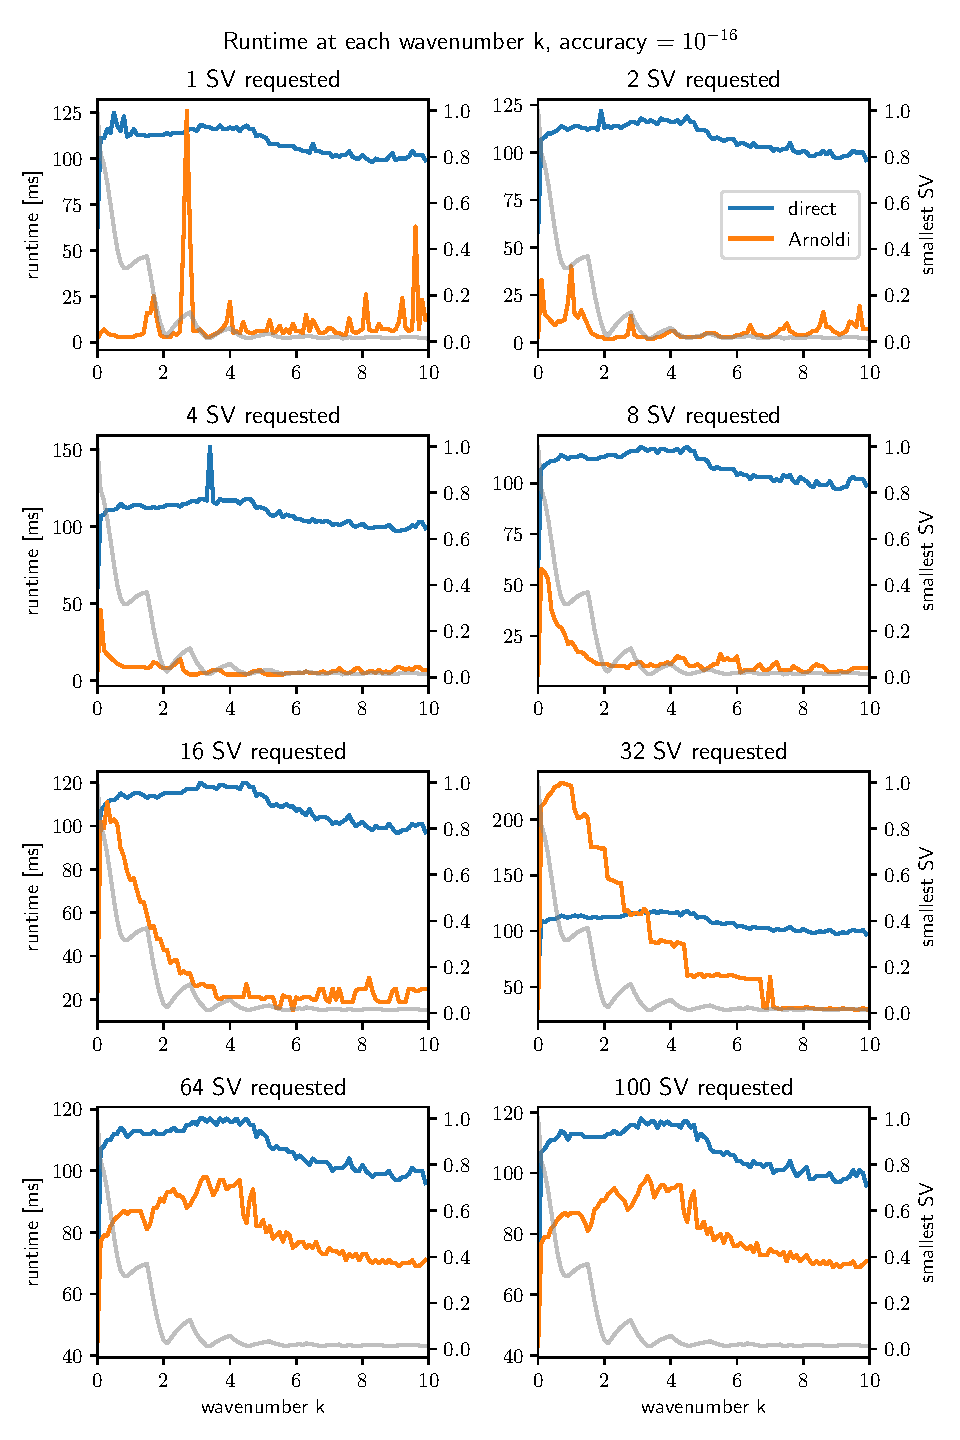
\includegraphics[width=\columnwidth]{figures/arnoldi_time_1e-16.pdf}
	\caption{
		The best speedup of about 15 occurs when requesting 2 singular values corresponding to 4 eigenvalues of the Wielandt matrix. 
		Here the cost of the extra $(matrix\times vector)$ products is less than what is gained through reducing the spikes that occur due to the bunching of the singular values.
	}
	\label{fig:arnoldi_time_1e-16}
\end{figure}
\begin{figure} [H]
	\centering
	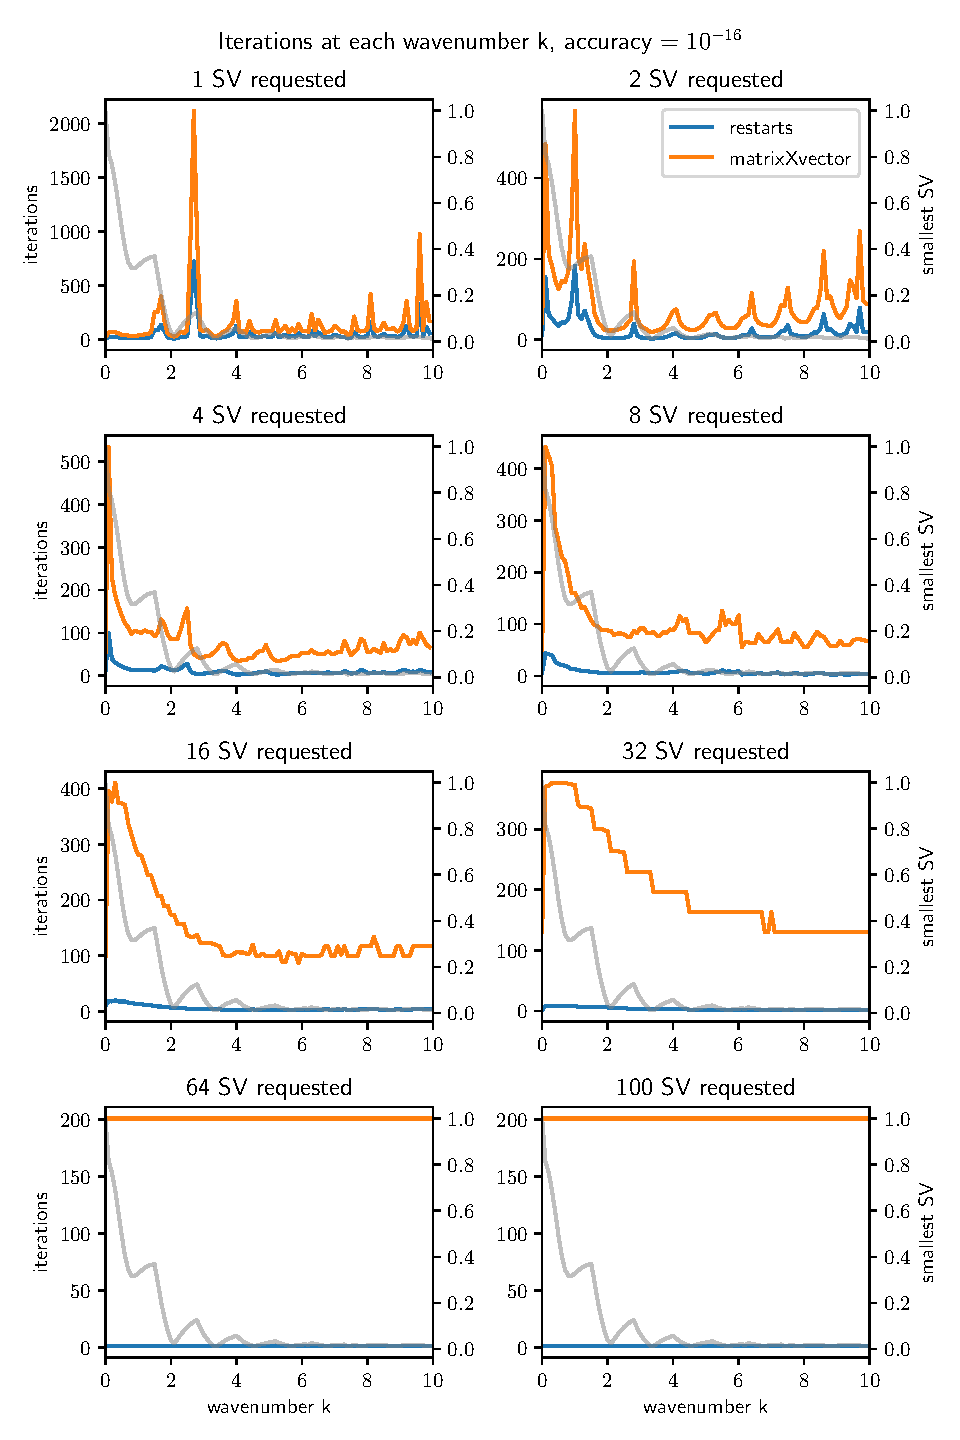
\includegraphics[width=\columnwidth]{figures/arnoldi_iter_1e-16.pdf}
	\caption{
		The iterations are proportional to the execution time and the number of $(matrix\times vector)$ products is proportional to the $\#restarts \times \#singularvalues$.
	}
	\label{fig:arnoldi_iter_1e-16}
\end{figure}

\section{Reduced Accuracy for Better Speedup}
In the last section we took the default parameters that were set by arpackpp.
This included an accuracy of $10^{-16}$, basically having us compute the eigenvalues precisely up to machine accuracy.
In order to see if we could reduce some of the iterations needed to come to convergence and therefore cut down on execution time we ran our root finding algorithm, using the Arnoldi method for computing the smallest eigenvalue and looked if we could get useful results with a less accurate solver. 
We searched for the root in the region were there was the first minima of the Scattering Transmission Problem for which we ran our experiment in the previous section.
The results can be seen in table \ref{tbl:red_acc}.
\begin{table}[h!]
	\centering
	\resizebox{\columnwidth}{!}{\begin{tabular}{ |c|c|c|c|c|c|c|c } 
			\hline
			accuracy & $10^{-16}$ & $10^{-8}$ & $10^{-4}$ & $10^{-2}$ & $10^{-1}$ & $10^{0}$  \\ 
			\hline
			minima at & 0.849159 & 0.849159 & 0.849159 & 0.849177  & 0.847611 & 0.847611 \\ 
			\hline
			restarts & 11.32 & 5.88 & 3.2 & 2.0 & 1.08 & 1.0 \\ 
			\hline
			$(matrix\times vector)$  & 38.0 & 21.12 & 12.88  & 9.2 & 6.16 & 6.00   \\ 
			\hline
	\end{tabular}}
	\caption{Change in singular values against change in grid size.}
	\label{tbl:red_acc}
\end{table}

It is clear that the accuracy with which the Arnoldi algorithm is run can be reduced to at least $10^{-4}$ without loosing any accuracy in the found root.
This already reduces the average iterations taken until convergence substantially.
Reducing the accuracy of the Arnoldi algorithm even further we see that we start to lose some accuracy in the found roots.
Depending on how precisely we need to know these roots it can however still be worth it since we are still decreasing the amount of iterations while at least qualitatively retaining the correct solution.

\section{Spikes and Speedups with Lower Accuracy}
Since we saw that the execution time of the Arnoldi algorithm was directly related to the number of iterations taken until convergence was reached and since we also saw that we could reduce the necessary number of iterations by reducing the accuracy with which the singular values were computed, we reran the test from section \ref{sec:first_results} with an accuracy of $10^0$.
The results can be seen in \ref{fig:arnoldi_time_1e2} and \ref{fig:arnoldi_iter_1e2}.
A this accuracy the Arnoldi algorithm as implemented by arpackpp basically does not do a convergence check anymore and therefore always ends without doing any restarts.
This means there is no possibility of spikes occurring and the speedup increases heavily.

\begin{figure} [H]
	\centering
	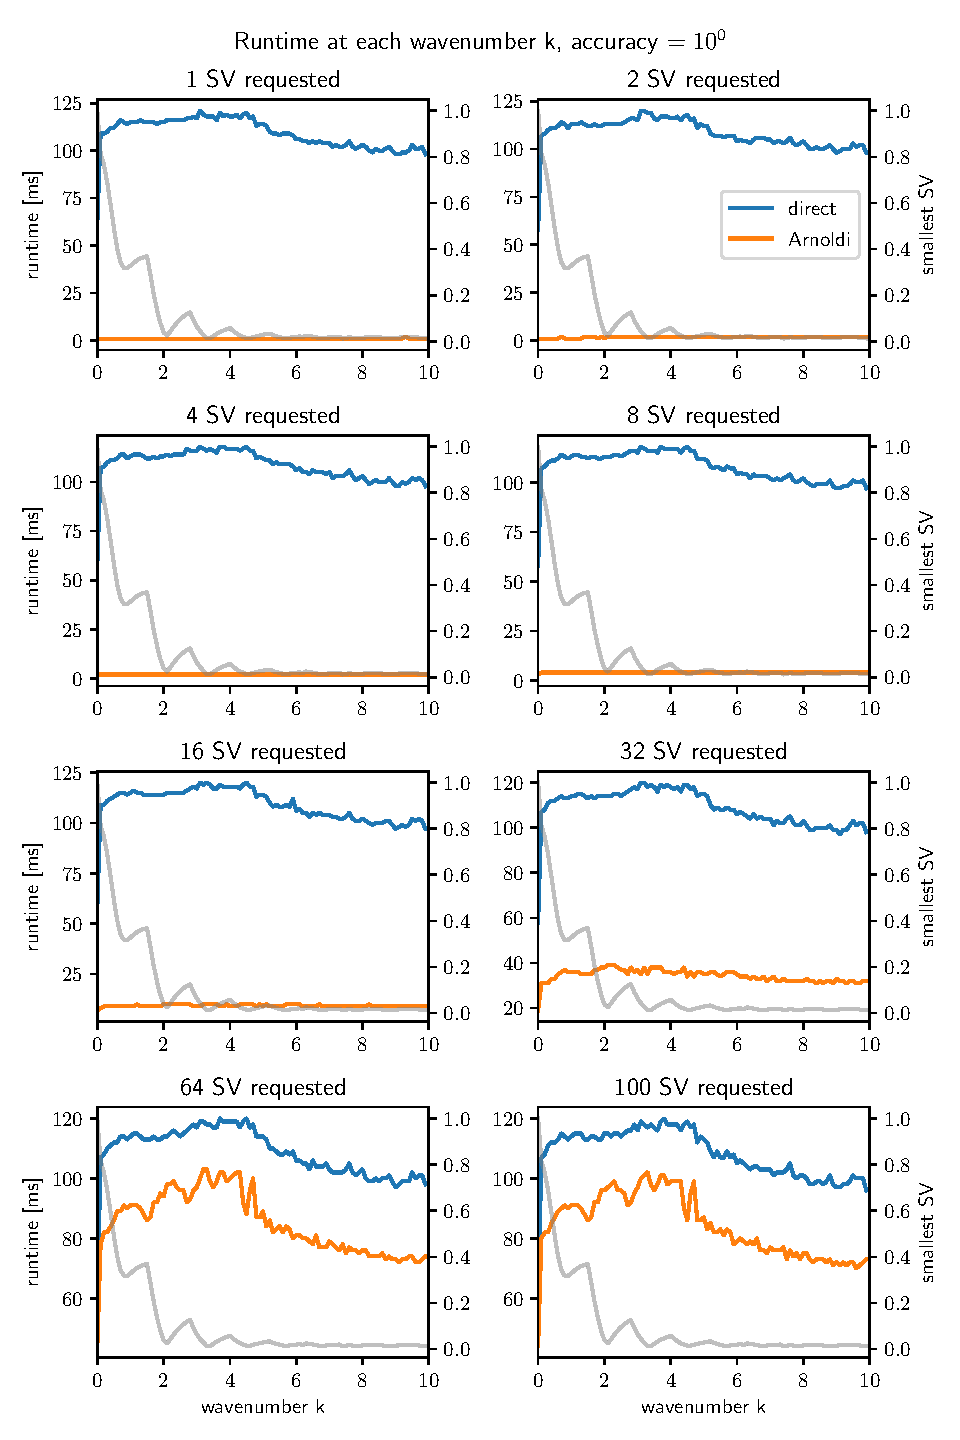
\includegraphics[width=\columnwidth]{figures/arnoldi_time_1e2.pdf}
	\caption{
		Without spikes the intuition of having the fastest execution time when requesting the fewest singular values becomes correct.
		This lead to having the highest speedup of about 100 fold for 1 requested eigenvalue when using the Arnoldi algorithm instead of the direct solver.
	}
	\label{fig:arnoldi_time_1e2}
\end{figure}
\begin{figure} [H]
	\centering
	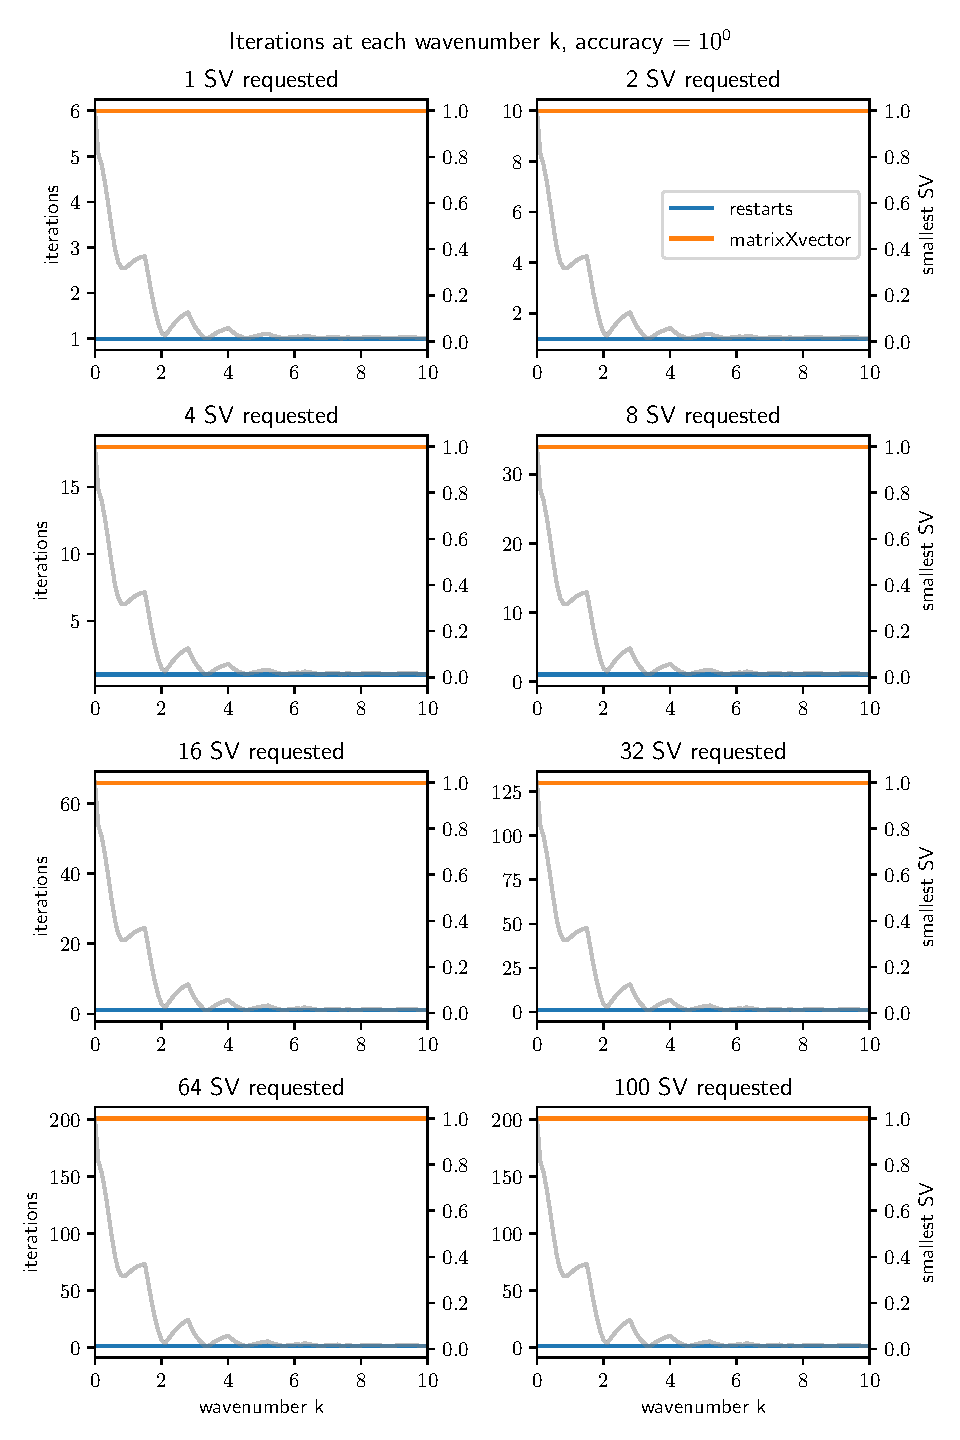
\includegraphics[width=\columnwidth]{figures/arnoldi_iter_1e2.pdf}
	\caption{
		Only one restart is done each time the Arnoldi algorithm is executed and the number of $(matrix\times vector)$ products is therefore proportional to the $\#singularvalues$.
	}
	\label{fig:arnoldi_iter_1e2}
\end{figure}

\end{document}

